\RequirePackage[l2tabu,orthodox]{nag}

% TODO: decide if one-sided/two-sided
%\documentclass[headsepline,footsepline,footinclude=false,fontsize=11pt,paper=a4,listof=totoc,bibliography=totoc,BCOR=12mm,DIV=12]{scrbook} % two-sided
\documentclass[headsepline,footsepline,footinclude=false,oneside,fontsize=11pt,paper=a4,listof=totoc,bibliography=totoc]{scrbook} % one-sided

\PassOptionsToPackage{table,svgnames,dvipsnames}{xcolor}

\usepackage[utf8]{inputenc}
\usepackage[T1]{fontenc}
\usepackage[sc]{mathpazo}
\usepackage[USenglish,british,UKenglish,american]{babel}
\usepackage[autostyle]{csquotes}
\usepackage{graphicx}
\usepackage{scrhack} % necessary for listings package
\usepackage{listings}
\usepackage{lstautogobble}
\usepackage{tikz}
\usepackage{pgfplots}
\usepackage{pgfplotstable}
\usepackage{booktabs}
\usepackage[final]{microtype}
\usepackage{caption}
\usepackage{subcaption}
% \usepackage[hidelinks]{hyperref} % hidelinks removes colored boxes around references and links
\usepackage{hyperref} % linkes with colored boxes
\usepackage{xspace}
\usepackage{booktabs,siunitx,rotating}
\usepackage{pifont}
% \usepackage{footmisc}

\usepackage[printonlyused]{acronym}
\usepackage[acronym, automake, toc, nonumberlist]{glossaries}
\makeglossaries

\usepackage[%
backend=biber,
url=false,
style=alphabetic,
maxnames=4,
minnames=3,
maxbibnames=99,
giveninits,
uniquename=init]{biblatex}
%\addbibresource{bibliography.bib}
\bibliography{bibliography}


\setkomafont{disposition}{\normalfont\bfseries} % use serif font for headings
\linespread{1.05} % adjust line spread for mathpazo font

% Add table of contents to PDF bookmarks
\BeforeTOCHead[toc]{{\cleardoublepage\pdfbookmark[0]{\contentsname}{toc}}}

% Define TUM corporate design colors
% Taken from http://portal.mytum.de/corporatedesign/index_print/vorlagen/index_farben
\definecolor{TUMBlue}{HTML}{0065BD}
\definecolor{TUMSecondaryBlue}{HTML}{005293}
\definecolor{TUMSecondaryBlue2}{HTML}{003359}
\definecolor{TUMBlack}{HTML}{000000}
\definecolor{TUMWhite}{HTML}{FFFFFF}
\definecolor{TUMDarkGray}{HTML}{333333}
\definecolor{TUMGray}{HTML}{808080}
\definecolor{TUMLightGray}{HTML}{CCCCC6}
\definecolor{TUMAccentGray}{HTML}{DAD7CB}
\definecolor{TUMAccentOrange}{HTML}{E37222}
\definecolor{TUMAccentGreen}{HTML}{A2AD00}
\definecolor{TUMAccentLightBlue}{HTML}{98C6EA}
\definecolor{TUMAccentBlue}{HTML}{64A0C8}

% Settings for pgfplots
\pgfplotsset{compat=newest}
\pgfplotsset{
  % For available color names, see http://www.latextemplates.com/svgnames-colors
  cycle list={TUMBlue\\TUMAccentOrange\\TUMAccentGreen\\TUMSecondaryBlue2\\TUMDarkGray\\},
}

% Settings for lstlistings
\lstset{%
  basicstyle=\ttfamily,
  columns=fullflexible,
  autogobble,
  keywordstyle=\bfseries\color{TUMBlue},
  stringstyle=\color{TUMAccentGreen}
}


% beautifully typesetted abbrevs.

% Add a period to the end of an abbreviation unless there's one
% already, then \xspace.
% taken from cvpr.sty
\makeatletter
\DeclareRobustCommand\onedot{\futurelet\@let@token\@onedot}
\def\@onedot{\ifx\@let@token.\else.\null\fi\xspace}
\DeclareRobustCommand\onecomma{\futurelet\@let@token\@onecomma}
\def\@onecomma{\ifx\@let@token,\else,\null\fi\xspace}

\def\eg{e.g.\onecomma} %\def\Eg{E.g.\onecomma}
\def\ie{i.e.\onecomma} %\def\Ie{I.e.\onecomma}
\def\cf{cf\onedot} \def\Cf{Cf\onedot}
\def\etc{\emph{etc}\onedot} \def\vs{vs\onedot}
\def\wrt{w.r.t\onedot} \def\dof{d.o.f\onedot}
\def\etal{\emph{et~al}\onedot}

\newcommand{\cmark}{\ding{51}}%
\newcommand{\xmark}{\ding{55}}%

\makeatother
% 
\makeglossaries

\newglossaryentry{duck}{name=duck,%
	description={a waterbird with webbed feet}}

\newglossaryentry{parrot}{name=parrot,%
	description={mainly tropical bird with bright plumage}}



\newcommand*{\getUniversity}{University of Applied Sciences Munich}
\newcommand*{\getFaculty}{Department of Computer Science and Mathematics}
\newcommand*{\getTitle}{On the generalization capabilities of interactive segmentation methods}
\newcommand*{\getTitleGer}{}
\newcommand*{\getAuthor}{Alexander Fertig}
\newcommand*{\getDoctype}{Master's Thesis in Computer Science}
\newcommand*{\getSupervisor}{Prof. Dr. David Spieler}
\newcommand*{\getAdvisor}{Advisor}
\newcommand*{\getSubmissionDate}{Submission date}
\newcommand*{\getSubmissionLocation}{Munich}
\newcommand{\Unit}[1]{\thinspace #1}

%\includeonly{chapters/03_chapter03/chapter3}
\begin{document}
	
% Set page numbering to avoid "destination with the same identifier has been already used" warning for cover page.
% (see https://en.wikibooks.org/wiki/LaTeX/Hyperlinks#Problems_with_Links_and_Pages).
\pagenumbering{alph}
\begin{titlepage}
  % HACK for two-sided documents: ignore binding correction for cover page.
  % Adapted from Markus Kohm's KOMA-Script titlepage=firstiscover handling.
  % See http://mirrors.ctan.org/macros/latex/contrib/koma-script/scrkernel-title.dtx,
  % \maketitle macro.
  \oddsidemargin=\evensidemargin\relax
  \textwidth=\dimexpr\paperwidth-2\evensidemargin-2in\relax
  \hsize=\textwidth\relax

  \centering

  \IfFileExists{logos/tum.pdf}{%
    \includegraphics[height=20mm]{logos/tum.pdf}
  }{%
    \vspace*{20mm}
  }

  \vspace{5mm}
  {\huge\MakeUppercase{\getFaculty{}}}\\

  \vspace{5mm}
  {\large\MakeUppercase{\getUniversity{}}}\\

  \vspace{20mm}
  {\Large \getDoctype{}}

  \vspace{15mm}
  {\huge\bfseries \getTitle{}}

  \vspace{15mm}
  {\LARGE \getAuthor{}}

  \IfFileExists{logos/faculty.pdf}{%
    \vfill{}
    \includegraphics[height=20mm]{logos/faculty.pdf}
  }{}
\end{titlepage}


\frontmatter{}
% import also possible with input, but then "\includeonly{}" is not applieable
\begin{titlepage}
  \centering
  
  \IfFileExists{logos/hm_logo_full_2020.pdf}{%
 	\vfill{}
	 
\includegraphics[height=30mm]{logos/hm_logo_full_2020.pdf}
	}{%
	\vspace*{30mm}
	}

  \vspace{15mm}
  {\huge\MakeUppercase{\getFaculty{}}}\\

  \vspace{5mm}
  {\large\MakeUppercase{\getUniversity{}}}\\

  \vspace{20mm}
  {\Large \getDoctype{}}

  \vspace{15mm}
  {\huge\bfseries \getTitle{} \par}

  \vspace{10mm}
  {\huge\bfseries \foreignlanguage{ngerman}{\getTitleGer{}} \par}

  \vspace{15mm}
  \begin{tabular}{l l}
    Author:          	& \getAuthor{} \\
    Matrikelnumber:	 	& \getMatrikelNum{} \\
    Study:			 	& Master Computer Science \\
    Supervisor:      	& \getSupervisor{}  \\
    Second Supervisor:	& \getSecondSupervisor{} \\
    Advisor:         	& \getAdvisor{} (MVTec Software GmbH)\\
    Submission Date: 	& \getSubmissionDate{} \\
  \end{tabular}

 
\end{titlepage}

\thispagestyle{empty}
\vspace*{0.75\textheight}
\noindent

I confirm that I have written the \MakeLowercase{\getDoctype{}} independently, have not submitted it elsewhere for examination purposes, have not used any sources or aids other than those referenced, and have marked literal and analogous quotations as such.

\vspace{15mm}
\noindent
\getSubmissionLocation{}, \getSubmissionDate{} \hspace{50mm} \getAuthor{}

\cleardoublepage{}

\addcontentsline{toc}{chapter}{Acknowledgments}
%\thispagestyle{empty}

\vspace*{20mm}

\begin{center}
{\usekomafont{chapter} Acknowledgments}

Matthias Klatt

Patrick Follmann

Benchmark Participants

MVTec
\end{center}

\vspace{10mm}


\cleardoublepage{}

\chapter{\abstractname}

%TODO: Abstract




% Don’t use \glsin chapter or section headings as it can have some unpleasantside-effects. Instead use \glsentrytextfor regular entries and one of \glsentryshort, \glsentrylong or \glsentryfull for acronyms. Alternatively useglossaries-extrawhich provides special commands for use insection headings and captions, such as \glsfmtshort{〈label〉}

% Apply in text:
% gls{}
% glspl{} --> plural form with 's'

\newacronym{cd}{CD}{compact disk}
\newacronym{gpu}{GPU}{Graphical Processing Unit}


\newacronym{dl}{DL}{Deep Learning}
\newacronym{ml}{ML}{Machine Learning}
\newacronym{ai}{AI}{Artificial Intellegence}
	
\newacronym{cnn}{CNN}{Convolutional Neural Network}
\newacronym{rnn}{RNN}{Recurrent Neural Network}
\newacronym{gcn}{GCN}{Graph Convolutional Network}

\newacronym{gt}{GT}{Ground Truth}
\newacronym{iou}{IoU}{Intersection over Union}
\newacronym{miou}{mIoU}{mean Intersection over Union}
\newacronym{op}{OP}{Overall Pixel}
\newacronym{pc}{PC}{Per-Class}
\newacronym{ap}{AP}{Average Precision}
	
\newacronym{ifcn}{iFCN}{interactive Fully Convolutional Network}
\newacronym{fctsfn}{FCTSFN}{Fully Convolutional Two-Stream Fusion Network}
\newacronym{itis}{ITIS}{Iterativly Trained Interative Segmentation}
\newacronym{risnet}{RIS-Net}{Regional Interactive Segmentation Network}
\newacronym{iog}{IOG}{Inside Outside Guidance}
\newacronym{dextr}{DEXTR}{Deep Extreme Cut}
\newacronym{fcn}{FCN}{Fully Convolutional Network}
\newacronym{psp}{PSP}{Pyramid Scene Parsing}
\newacronym{crf}{CRF}{Conditional Random Fields}
\newacronym{spp}{SPP}{Spatial Pyramid Pooling}
\newacronym{aspp}{ASPP}{Atrous Spatial Pyramid Pooling}


\microtypesetup{protrusion=false}
\setcounter{tocdepth}{1}
\tableofcontents{}
\microtypesetup{protrusion=true}

\mainmatter{}


% % !TeX root = ../main.tex
% Add the above to each chapter to make compiling the PDF easier in some editors.

\chapter{Example-Chapter}\label{chapter:introduction}

\section{Example-Section}
Citation test~\parencite{latex} \cite{Zha2020}.

\subsection{Example-Subsection}

See~\autoref{tab:sample}, \autoref{fig:sample-drawing}, \autoref{fig:sample-plot}, \autoref{fig:sample-listing}.

\begin{table}[htpb]
  \caption[Example table]{An example for a simple table.}\label{tab:sample}
  \centering
  \begin{tabular}{l l l l}
    \toprule
      A & B & C & D \\
    \midrule
      1 & 2 & 1 & 2 \\
      2 & 3 & 2 & 3 \\
    \bottomrule
  \end{tabular}
\end{table}

\begin{figure}[htpb]
  \centering
  % This should probably go into a file in figures/
  \begin{tikzpicture}[node distance=3cm]
    \node (R0) {$R_1$};
    \node (R1) [right of=R0] {$R_2$};
    \node (R2) [below of=R1] {$R_4$};
    \node (R3) [below of=R0] {$R_3$};
    \node (R4) [right of=R1] {$R_5$};

    \path[every node]
      (R0) edge (R1)
      (R0) edge (R3)
      (R3) edge (R2)
      (R2) edge (R1)
      (R1) edge (R4);
  \end{tikzpicture}
  \caption[Example drawing]{An example for a simple drawing.}\label{fig:sample-drawing}
\end{figure}

\begin{figure}[htpb]
  \centering

  \pgfplotstableset{col sep=&, row sep=\\}
  % This should probably go into a file in data/
  \pgfplotstableread{
    a & b    \\
    1 & 1000 \\
    2 & 1500 \\
    3 & 1600 \\
  }\exampleA
  \pgfplotstableread{
    a & b    \\
    1 & 1200 \\
    2 & 800 \\
    3 & 1400 \\
  }\exampleB
  % This should probably go into a file in figures/
  \begin{tikzpicture}
    \begin{axis}[
        ymin=0,
        legend style={legend pos=south east},
        grid,
        thick,
        ylabel=Y,
        xlabel=X
      ]
      \addplot table[x=a, y=b]{\exampleA};
      \addlegendentry{Example A};
      \addplot table[x=a, y=b]{\exampleB};
      \addlegendentry{Example B};
    \end{axis}
  \end{tikzpicture}
  \caption[Example plot]{An example for a simple plot.}\label{fig:sample-plot}
\end{figure}

\begin{figure}[htpb]
  \centering
  \begin{tabular}{c}
  \begin{lstlisting}[language=SQL]
    SELECT * FROM tbl WHERE tbl.str = "str"
  \end{lstlisting}
  \end{tabular}
  \caption[Example listing]{An example for a source code listing.}\label{fig:sample-listing}
\end{figure}

% !TeX root = ../../main.tex
% Add the above to each chapter to make compiling the PDF easier in some editors.

\chapter{Introduction}\label{chapter:chapter1}

%% !TeX root = ../../main.tex
% Add the above to each chapter to make compiling the PDF easier in some editors.

\section{Section}\label{ord:ch1:sec1}
Citation test~\parencite{latex} \cite{Zha2020}.

\subsection{Subsection}\label{ord:ch1:subsec1}

See~\autoref{tab:ch1:sample}, \autoref{fig:ch1:sample-drawing}, \autoref{fig:ch1:sample-plot}, \autoref{fig:ch1:sample-listing}.

\begin{table}[htpb]
  \caption[Example table]{An example for a simple table.}\label{tab:ch1:sample}
  \centering
  \begin{tabular}{l l l l}
    \toprule
      A & B & C & D \\
    \midrule
      1 & 2 & 1 & 2 \\
      2 & 3 & 2 & 3 \\
    \bottomrule
  \end{tabular}
\end{table}

\begin{figure}[htpb]
  \centering
  % This should probably go into a file in figures/
  \begin{tikzpicture}[node distance=3cm]
    \node (R0) {$R_1$};
    \node (R1) [right of=R0] {$R_2$};
    \node (R2) [below of=R1] {$R_4$};
    \node (R3) [below of=R0] {$R_3$};
    \node (R4) [right of=R1] {$R_5$};

    \path[every node]
      (R0) edge (R1)
      (R0) edge (R3)
      (R3) edge (R2)
      (R2) edge (R1)
      (R1) edge (R4);
  \end{tikzpicture}
  \caption[Example drawing]{An example for a simple drawing.}\label{fig:ch1:sample-drawing}
\end{figure}

\begin{figure}[htpb]
  \centering

  \pgfplotstableset{col sep=&, row sep=\\}
  % This should probably go into a file in data/
  \pgfplotstableread{
    a & b    \\
    1 & 1000 \\
    2 & 1500 \\
    3 & 1600 \\
  }\exampleA
  \pgfplotstableread{
    a & b    \\
    1 & 1200 \\
    2 & 800 \\
    3 & 1400 \\
  }\exampleB
  % This should probably go into a file in figures/
  \begin{tikzpicture}
    \begin{axis}[
        ymin=0,
        legend style={legend pos=south east},
        grid,
        thick,
        ylabel=Y,
        xlabel=X
      ]
      \addplot table[x=a, y=b]{\exampleA};
      \addlegendentry{Example A};
      \addplot table[x=a, y=b]{\exampleB};
      \addlegendentry{Example B};
    \end{axis}
  \end{tikzpicture}
  \caption[Example plot]{An example for a simple plot.}\label{fig:ch1:sample-plot}
\end{figure}

\begin{figure}[htpb]
  \centering
  \begin{tabular}{c}
  \begin{lstlisting}[language=SQL]
    SELECT * FROM tbl WHERE tbl.str = "str"
  \end{lstlisting}
  \end{tabular}
  \caption[Example listing]{An example for a source code listing.}\label{fig:ch1:sample-listing}
\end{figure}

% !TeX root = ../../main.tex
% Add the above to each chapter to make compiling the PDF easier in some editors.

\section{Section}\label{ord:ch1:sec1}

\subsection{Subsection}\label{ord:ch1:sec1:subsec1}

See~\autoref{tab:ch1:sample}, \autoref{fig:ch1:sample-drawing}, \autoref{fig:ch1:sample-plot}, \autoref{fig:ch1:sample-listing}.

\begin{table}[htpb]
  \caption[Example table]{An example for a simple table.}\label{tab:ch1:sample}
  \centering
  \begin{tabular}{l l l l}
    \toprule
      A & B & C & D \\
    \midrule
      1 & 2 & 1 & 2 \\
      2 & 3 & 2 & 3 \\
    \bottomrule
  \end{tabular}
\end{table}

\begin{figure}[htpb]
  \centering
  % This should probably go into a file in figures/
  \begin{tikzpicture}[node distance=3cm]
    \node (R0) {$R_1$};
    \node (R1) [right of=R0] {$R_2$};
    \node (R2) [below of=R1] {$R_4$};
    \node (R3) [below of=R0] {$R_3$};
    \node (R4) [right of=R1] {$R_5$};

    \path[every node]
      (R0) edge (R1)
      (R0) edge (R3)
      (R3) edge (R2)
      (R2) edge (R1)
      (R1) edge (R4);
  \end{tikzpicture}
  \caption[Example drawing]{An example for a simple drawing.}\label{fig:ch1:sample-drawing}
\end{figure}

\begin{figure}[htpb]
  \centering

  \pgfplotstableset{col sep=&, row sep=\\}
  % This should probably go into a file in data/
  \pgfplotstableread{
    a & b    \\
    1 & 1000 \\
    2 & 1500 \\
    3 & 1600 \\
  }\exampleA
  \pgfplotstableread{
    a & b    \\
    1 & 1200 \\
    2 & 800 \\
    3 & 1400 \\
  }\exampleB
  % This should probably go into a file in figures/
  \begin{tikzpicture}
    \begin{axis}[
        ymin=0,
        legend style={legend pos=south east},
        grid,
        thick,
        ylabel=Y,
        xlabel=X
      ]
      \addplot table[x=a, y=b]{\exampleA};
      \addlegendentry{Example A};
      \addplot table[x=a, y=b]{\exampleB};
      \addlegendentry{Example B};
    \end{axis}
  \end{tikzpicture}
  \caption[Example plot]{An example for a simple plot.}\label{fig:ch1:sample-plot}
\end{figure}

\begin{figure}[htpb]
  \centering
  \begin{tabular}{c}
  \begin{lstlisting}[language=SQL]
    SELECT * FROM tbl WHERE tbl.str = "str"
  \end{lstlisting}
  \end{tabular}
  \caption[Example listing]{An example for a source code listing.}\label{fig:ch1:sample-listing}
\end{figure}

% !TeX root = ../../main.tex
% Add the above to each chapter to make compiling the PDF easier in some editors.

\chapter{Theory}\label{ord:ch2}

% !TeX root = ../../main.tex
% Add the above to each chapter to make compiling the PDF easier in some editors.

\section{Basics}\label{ord:ch2:sec1}

In the last decade the development and research interest in the field of \gls{ml} have greatly increased and drawn much attention. 
This section briefly recaptures the fundamental concepts of \gls{ml} and \gls{dl}.
A detailed description of the introduced concepts and terms can be reviewed in \cite{Ger17-HandsOn} or \cite{Goodfellow-et-al-2016}.

%The last decade was revolutionary for the sector of information technology.
%Due to technical advancement, the computational power of processors, especially \gls{gpu} rise significantly.
%Further, the wider creation and use of data introduced the domain of big data, that allows operators to gain more insights and benefits.
%Both of these recent advancements benefited another field of study commonly described as \gls{ai}.
%The term \gls{ai} describes machines that are show characteristics of human intelligence that allow them to handle various tasks.
%But there are several gradations, that hide behind the powerful bus word \gls{ai} and are illustrated in this section.

\subsection{Machine Learning}\label{ord:ch2:sec1:subsec1}

\gls{ml} is the science of creating algorithms, to analyze, detect and learn patterns in various kinds of data without defining explicit decision rules.
These algorithms may achieve human level performance, but mostly they are limited to a single task.
In order to solve another task a \gls{ml} algorithm, has to learn the patterns of the new task from a corresponding dataset $\mathcal{D}$.
As \gls{ml} algorithms aim to model reality, they are also referred to as \gls{ml} model.

% Dataset 
The dataset $\mathcal{D}$ usually is split into a training set $\mathcal{S}$, a test set $\mathcal{S}_2$ and validation set $\mathcal{S}_3$.
These three types of datasets are treated separately, while the \gls{ml} model uses the training set $\mathcal{S}$ to extract the patterns, the test set $\mathcal{S}_2$ and validation set $\mathcal{S}_3$ are only used to evaluate the performance of the model.

% Input x and label y
A dataset $\mathcal{D}$ contains $N$ elements with each element having $M$ features.
An element $\textbf{x}$ can be represented as feature-vector $\textbf{x} = [x_1, \dots ,x_M]$, which the model takes as input.
For the task of supervised learning, the dataset $\mathcal{D}$ consists out of pairs $(\textbf{x}_n, y_n)$. Each input $\textbf{x}_i$ contains a corresponding label $y_i$.
In the scope of classification, this label $y$ is represented by one out of $K$ classes $y \in \lbrace c_1, \dots, c_K \rbrace$.
The classification task is defined as  
\begin{equation}
	f: \mathbb{R}^M \rightarrow \lbrace c_1,\ldots,c_K \rbrace, \quad \textbf{x} \mapsto y
\end{equation}
In order to create a functioning model, the model is trained by adjusting it's inner parameters, referred to as $ \theta $ the weights of the model.
While training a model, the weights are adjusted based on the features are extracted iteratively from the given input $\textbf{x}$.

% Model prediction
The function $f$ describes the model, which computes the estimated output $\hat{y}$ based on the input $\textbf{x}$
\begin{equation}
	\hat y = f(\textbf{x}, \theta)
\end{equation}
with $\hat{y}$ being also referred to as prediction of the model and $ \theta $ as the weights of the model.

% Loss function and Backpropagation
In order to perform a training, the model requires a loss function $L(y,\hat{y})$.
The loss function $L$ calculates the loss of the model based on the difference of the prediction $\hat{y}$ and the true label $y$.
There exist different loss functions to calculate various types of losses.
Depending on the loss the weights of the model are adjusted, to make a better prediction and reduce the error.
Usually, an algorithm called backpropagation \cite{Lin76-Backprob} is used to derive the gradient of the loss with respect to all the weights of the model.
With this, \gls{sgd} can be used to iteratively update the weights and optimize the model.
In the context of \gls{ml} the term \textit{learning} refers to this process.

% Generalization error of a model
The goodness of a model can be defined by the performance on the training set $\mathcal{S}$, test set $\mathcal{S}_2$, and validation set $\mathcal{S}_3$.
The two main causes of failure are underfitted or overfitted models.
An underfitted model is not complex enough to understand the interrelations in the data and therefore, does not perform well.
Common reasons for underfitted models are missing complexity in the model architecture or too small and not representative datasets.
Overfitted models perform great on the training set $\mathcal{S}$, but poorly on the test set $\mathcal{S}_2$ and validation set $\mathcal{S}_3$.
This happens, when the model does not generalize well enough and instead learns the features of the training set by heart.
To successfully train a model, a tradeoff between overfitting and underfitting must be found.

% Hyperparameter
Further, there exist so-called \textit{hyperparameters}, that are used to adjust the training process or the model architecture.
Important hyperparameters are the learning rate $\lambda$ , the number of training epochs $N_{Epochs}$, and the applied optimizer.


\subsection{Deep Learning}\label{ord:ch2:sec1:subsec2}

For this thesis, it is assumed that the reader is already familiar with the field of \gls{dl}. 
If this is not the case, \cite{Goodfellow-et-al-2016} and \cite{Ger17-HandsOn} provide a detailed introduction to this topic.
A \gls{nn} is one of the standard \gls{ml} methods and consists out of multiple neurons.
The architecture principle is characterized by layer-wise order of the neurons.
Similar as for basic \gls{ml} models, a \gls{nn} processes an input $ \textbf{x} $ to create a prediction $ \hat{y} $, which for the task of classification is a class $ c_i $.
If an architecture consists out of multiple layers, the network is also described as \textit{deep}, resulting in the terms \gls{dl} and \gls{dnn}.
The neurons are connected layer by layer, each neuron receives $ n $ inputs $ \left[\textbf{x}_1, \dots \textbf{x}_n \right] $ from the previous layer and passes the output to the next layer.
A neuron sums its input values and applies an activation function to create an output, a frequently used activation function is the \gls{relu} function, an overview is provided in \Cite{SSA20-Activationfunctions}. 

Each connection between neurons is weighted, which determines the relevance of the input $ \textbf{x}_i $ for the individual neuron.
This is done by weights $ \theta $, which are adjusted during the training as the model is in the \textit{learning} process as described previously.

Nowadays, in order to solve various tasks, a variety of different network types exist \eg convolutional, graph or recurrent neural networks.
For the popular task of image processing \glspl{cnn} have proven themselves to be most adequate to classify, localize, or segment objects in images.
The main component of \glspl{cnn} are convolutional layers, that are used to process and extract features from visual input.
In these layers a convolution operation is performed on the input by applying $c$ convolution kernels.
The output of a layer is defined as a feature map $F_c$, with also $c$ representing the amount of channels in the feature map.
Further, pooling layers are commonly used, in order to reduce the size of feature maps.
% TODO example image of CNN

\subsection{Evaluation}\label{ord:ch2:sec1:subsec3}

The performance of a model may be evaluated using various metrics.
In the context of classification, the \textit{true positives} are the number of instances, that are correctly predicted to belong to a certain class $c_i$.
While the \textit{false positives} are the number of instances, that are incorrectly predicted to be positive, but truly are negative.
The contradictory definition applies for the equivalent terms \textit{true negatives} and \textit{false negatives}.

% Accuracy
%\begin{equation}
%	Accuracy = \frac{\textnormal{\textit{true positives}} + \textnormal{\textit{true negatives}}}{\textnormal{\textit{true positives}} + \textnormal{\textit{false positives}} + \textnormal{\textit{true negatives}} + \textnormal{\textit{false negatives}}}
% \end{equation}
The accuracy is one of the most simple metrics and represents the number of correct predictions over the number of all predictions.
To further gain deeper insights on the behavior of models there exist more evaluation metrics as precision and recall \cite{Ger17-HandsOn}.
% precision
%The precision is defined by
%\begin{equation}
%	precision = \frac{\textnormal{\textit{true positives}}}{\textnormal{\textit{true positives}} + \textnormal{\textit{false positives}}}
%\end{equation}
%and represents the accuracy of the positive predictions.
% recall
%The recall is defined by
%\begin{equation}
%	recall = \frac{\textnormal{\textit{true positives}}}{\textnormal{\textit{true positives}} + \textnormal{\textit{false negatives}}}
%\end{equation}
%and is also referred to as \textit{sensitivity} or \textit{true positve rate}.
%The recall describes the ratio of positive instances, that are predicted correctly \cite{Ger17-HandsOn}.

% Further, there exist methods for the evaluation of model as the \textit{F1-Score} or the ROC curve, that are described in \cite{Ger17-HandsOn}.
% !TeX root = ../../main.tex
% Add the above to each chapter to make compiling the PDF easier in some editors.

\section{Semantic Segmentation}\label{ord:ch2:sec2}

\subsection{Motivation}\label{ord:ch2:sec2:subsec_motivation}
Semantic segmentation finds application in various tasks and is widely used over different domains.
Due to its capability to perform classification on pixel-level it is often applied on scene understanding \cite{LiJ09-SceneUnderstanding} or the evaluation of satellite images \cite{Li18-SateliteImagery}.
In the field of autonomous driving semantic segmentation is used for street scene analysis \cite{Cor16-Cityscapes} \cite{Men15-AutonVehicles} \cite{Neu17-MapillaryDataset}.
In medicine this method can be used to segment cancer cells, tumors \cite{RF15-U-Net} or blood cells \cite{Tran19-BloodCell}.
Further, it is applied in order to fulfill abstract tasks like the reconstruction of indoor scenes \cite{Dai17-ReconstructionIndoorScenes}.
This listing of only some applications gives an idea of how versatile and functional image segmentation is and what can be achieved with it in the future.


\subsection{General}\label{ord:ch2:sec2:subsec_general}
Image segmentation is an advanced task of computer vision.
The goal of segmentation algorithms is to obtain regions of interest from an image.
In order to partition the image into regions, a high level of understanding is required.
Modern techniques of \gls{dl} have proven themselves to be most adequate for this task.
For image segmentation nowadays deep \glspl{cnn} are applied.
There two main variants to perform segmentation on images:
\begin{itemize}
	% Semantic segmentation
	\item \textbf{Semantic segmentation} classifies each pixel with one class \cite{RF15-U-Net} \cite{Zhao17-PSP}, illustrated in Figure \ref{fig:ch2:sec2:semantic_seg}.
	There is no differentiation made if there are multiple objects of one class, they all belong to the same region.
	% Instance segmentation
	\item \textbf{Instance segmentation} differentiates between different objects object instances \cite{DHS16-MNC} \cite{He17-MaskR-CNN} as shown in Figure \ref{fig:ch2:sec3:instance_seg}.
	Each instance has its own region and a label of the corresponding class $k$.
	In the result several regions may have the same class, but are treated as independent instances of this class.
\end{itemize}

This thesis deals with the labeling of objects and therefore it is further not distinguished between semantic and instance segmentation.
This is why, the labeling process of an instance may also be seen as semantic segmentation on a limited domain.
\begin{figure} [h]
	\centering
	\begin{subfigure}[t]{0.3\textwidth}
		\centering
		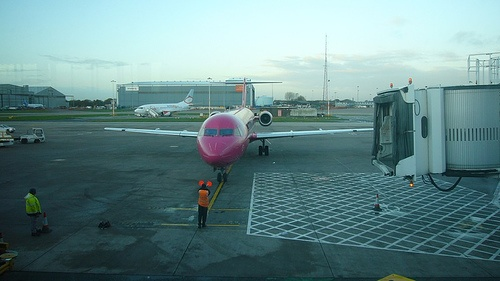
\includegraphics[width=\textwidth]{figures/chap22_image.jpg}
		\caption{
			Input image $\textbf{x}$
		}\label{fig:ch2:sec2:image}
	\end{subfigure}
	\hfill
	\begin{subfigure}[t]{0.3\textwidth}
		\centering
		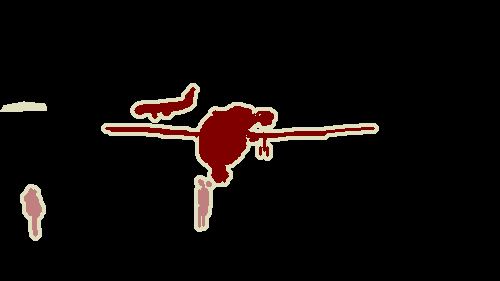
\includegraphics[width=\textwidth]{figures/chap22_semantic_seg.png}
		\caption{
			\gls{gt} for semantic segmentation.
			Each class has a label of the same color.
		} \label{fig:ch2:sec2:semantic_seg}
	\end{subfigure}
	\hfill
	\begin{subfigure}[t]{0.3\textwidth}
		\centering
		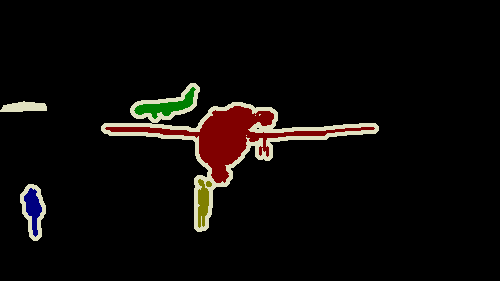
\includegraphics[width=\textwidth]{figures/chap22_instance_seg.png}
		\caption{
			\gls{gt} for instance segmentation.
			Each instance has a different colored label.
		}\label{fig:ch2:sec3:instance_seg}
	\end{subfigure}
	\caption[Semantic and instance segmentation]{
		Sample images of the PASCAL \glsentryshort{voc} Dataset \cite{Eve20-PascalVOC}, that distinguish between semantic and instance segmentation.
		The background class is colored back.
		The white class are the void pixel, that are around boundary of the object.
	}\label{fig:ch2:sec2:segmentation_image}
\end{figure}

% Supervised-learning, data with labels on pixel-level.
This thesis concentrates on methods of supervised learning.
Therefore, a dataset with labels for each image on pixel-level is required.
A label $y$ is represented by a map, which is an image of the same size as the input image $\textbf{x}$ and where each pixel has class label $y_{rc}$ with $r$ and $c$ referring to the corresponding row and column of the map. 
In this context the label $y$ is also referred to as mask or \gls{gt}.
Segmentation is treated as a classification task with $K$ classes.
The model creates a prediction $\hat{y}$, that also represented by a map, similar to the map $y$.
In this map a class $k$ is predicted for each pixel $\hat{y}_{rc}$.
Pixels with a the same class label form a region, that may be further processed afterwards.

% Loss function.
To train a segmentation network a loss function is required, that considers the loss of every pixel in the image and optimizes the prediction for each pixel individually.
In \cite{Jad20-LossFunction} several loss functions for image segmentation are examined.
Jadon concludes, that there is no universal loss function, instead their performance depends on the characteristics of the dataset.
Cross entropy loss works best on a balanced dataset, while for imbalanced datasets the dice coefficient or focal loss is suitable.

% TODO introductional sentence that this is important for the architecture???
The task of semantic segmentation aims to answer the questions of classification \emph{what is in the image?} and the question of localization \emph{where is it in the image?}.
The network extracts features and learns to answer the question of classification.
During this process the size of feature maps decrease and localization information is lost.
As a result it gets harder to perform a detailed reconstruction and answers the question of localization.
Architectural solutions to solve to solve this problem are introduced in Section \ref{ord:ch2:sec2:subsec_arch}.

\paragraph{PASCAL VOC Dataset}

% Basic description
The PASCAL \glsentryfull{voc} Challenge \cite{Eve20-PascalVOC} is established as a frequently used benchmark for the tasks of image classification, detection, and segmentation.
Due to this variety in application, the PASCAL \gls{voc} Challenge enjoys great popularity in the \gls{dl} community.
From 2005 to 2012 an annual challenge was created with an annual advanced dataset.
Despite the last release is almost a decade ago, the PASCAL \gls{voc} 2012 dataset is still to evaluate state-of-the-art methods and is used a benchmark for comparisons.
Due to the large use in recent years, this dataset also plays an important role in this thesis.
A sample with image and labels from the PASCAL \gls{voc} 2012 dataset is shown in Figure \ref{fig:ch2:sec2:segmentation_image}
% Size (iamges and annots) and label types
For the task of segmentation this dataset contains 6,929 annotations from 20 classes.

% Some times questionable labels of bicycles and plants
Despite the PASCAL \gls{voc} 2012 dataset is fairly popular, it features certain disadvantages, which must be taken into account for a fair evaluation.
First, the quality of some single annotations is questionable.
It was experienced, that especially for thin, long objects (\eg plants or the spite of bicycle wheels) the \gls{gt} partly seems inaccurate.
% often used for evaluation -> careful because general use datatset
Second, the PASCAL \gls{voc} datasets have so-called \textit{void pixel}, that are located around each object as a boundary, as illustrated in Figure \ref{fig:ch2:sec2:segmentation_image}.
They were established to prevent the inclusion of wrongly labeled \gls{gt} pixels, as label inaccuracies especially take place around the boundary of the object.  
Void pixel are excluded from the training and evaluation, which leads to a distorted evaluation result.
In most comparisons the presented results on PASCAL \gls{voc} datasets are created with the application of void pixel.
This does not lead to a realistic evaluation, since the boundary, which is particularly difficult to segment, is ignored.
Evaluating the performance, this must be taken into account, because real world data do have void pixel. 
In Section \ref{ord:ch5:sec1}, experiments demonstrate, that the performance significantly drops without the use of void pixel.


\subsection{Evaluation Metric}\label{ord:ch2:sec2:subsec_metric}
To ensure an objective comparison of several methods a evaluation metric is required, which measures the quality of obtained segmentation.
% OP
As this challenge is a classification task on pixel-level, a measure of evaluation is the \gls{op} accuracy, which represents the proportion of all correctly labeled pixels in an image or a whole dataset.
% "One significant limitation of this measure is its bias in the presence of very imbalanced classes. This is the case for the background class on PASCAL VOC datasets, which covers 70-75% of all pixels" \cite{Csu13-EvalMetric}
% PC
Further, the \gls{op} measurement can be refined by calculating the accuracy for each class.
This results in the \gls{pc} accuracy, which represents the proportion of correctly labeled pixels of one class.
% AP
% Another metric is the \gls{ap} 
%Another common metric is the \textit{Precision}, which the accuracy of the positive predictions and defined as
%\begin{equation}
%	Precision = \frac{\textnormal{true positives}}{\textnormal{true positives} + \textnormal{ false positves}}
%\end{equation}

% IoU
The most commonly used evaluation metric is the \gls{iou}, also known as the Jaccard Index, which is used in the PASCAL VOC challenge \cite{Eve20-PascalVOC} since 2008 \cite{Csu13-EvalMetric}. 
The \gls{iou} measures the ratio of overlap (true positives) between \gls{gt} and prediction $\hat{y}$ and of the total area. 
It is defined as
\begin{equation} \label{equ:iou}
	\centering
	IoU = \frac{\textnormal{\textit{true positives}}}{\textnormal{\textit{true positives}} + \textnormal{\textit{false negatives}} + \textnormal{\textit{false positves}}}
\end{equation}
and is calculated for each instance or segmentation class.
To evaluate all instances or classes of an image or a dataset the \gls{iou} is averaged, which results in the \gls{miou}.\footnote{An open source implementation can be found, \eg in TensorFlow: \textit{tf.keras.metrics.MeanIoU}: \url{https://www.tensorflow.org/api_docs/python/tf/keras/metrics/MeanIoU}}
%TODO other reference here than open source stuff??

\begin{figure}
	\centering
	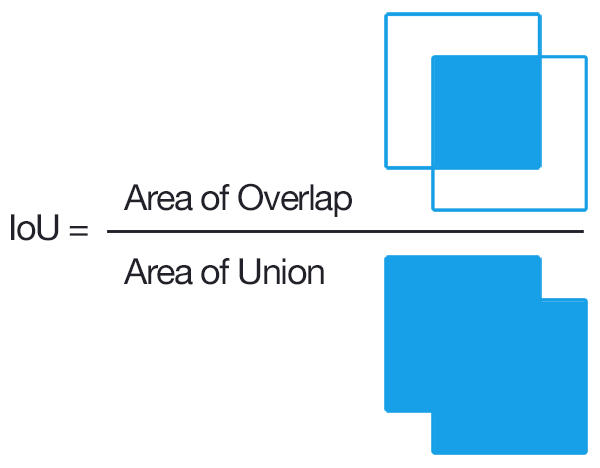
\includegraphics[width=0.5\textwidth]{figures/chap222_iou.png}
	\caption[Intersection over Union]{
		\glsentrylong{iou}. The \textit{area of overlap} represents the intersection of the \gls{gt} with the made prediction $\hat{y}$. 
		The \textit{area of union} represents the total area of \gls{gt} and the prediction $\hat{y}$ \cite{Sha18-DLCV}. \textit{TODO recreate a visualization like this by myself}}
	\label{fig:ch2:sec2:iou}
\end{figure}
% TODO get licence or change grafic 

An advantage of this metric is the inclusion of \textit{false positives} and \textit{false negatives} into the calculation.
A limitation of the \gls{iou} metric is that the boundary correctness of the region's boundaries is not taken into account. 
In order to compensate this issue, Csurka suggests in \cite{Csu13-EvalMetric} to combine the \gls{iou} with another complementary metric, evaluating the boundary of a region.
Regardless, the \gls{iou} is a suitable and informative metric, which is also the most common to evaluate semantic segmentation models.



\subsection{Semantic Segmentation Architectures}\label{ord:ch2:sec2:subsec_arch}
\gls{cnn} architectures for image classification follow a common scheme: 
A multi dimensional input image $\textbf{x}$ is processed and continuously downsized to a one dimensional tensor, in order to make one prediction $\hat{y}$.
In contrast, for image segmentation a prediction is made for each pixel of the image.
Therefore, an adaption of the architecture required, that enables the model to make a prediction for every pixel of the image $\hat{y}_{rc}$.
In the following characteristics of important architectures and components are examined.

\subsubsection{Encoder-Decoder-Architecture}
The Encoder-Decoder-Architecture as its name anticipates is based on two main parts: the encoder network and the decoder network, exemplary visualized in Figure \ref{fig:ch2:sec2:encoder-decoder}. 
Representatives of the encoder-decoder-architecture are U-Net \cite{RF15-U-Net}, DeConvNet \cite{NHH15-DeConvNet} and SegNet \cite{Bad17-SegNet}.

The encoder network is the feature extraction part of a classification \gls{cnn}.
It consists out of convolution and pooling layers, that reduce the size of the feature maps and extract features.
Therefore, the encoder network is the classification backbone and for DeConvNet \cite{NHH15-DeConvNet} and SegNet \cite{Bad17-SegNet} the backbone is based on VGG-16 \cite{SZ15-VGG16}. 
In this context the process of applying the encoder network is also called \textit{downsampling}, due to the size reduction of the feature maps.

The decoder network is the counterpart of the encoder network.
It reconstructs the feature maps to their original size, which is also referred to as \textit{upsampling}.
To reach the input size often a reversed architecture of the encoder network is used.
The basic components of this reconstruction are the operations \textit{unpooling} and \textit{transposed convolution}, introduced in the following.

After the encoder network generally a softmax classifier is applied, that predicts the class for each pixel.
The output is a probability map $\hat{y}$ with $K$ channels for $K$ number of classes \cite{Bad17-SegNet}.

\begin{figure}
	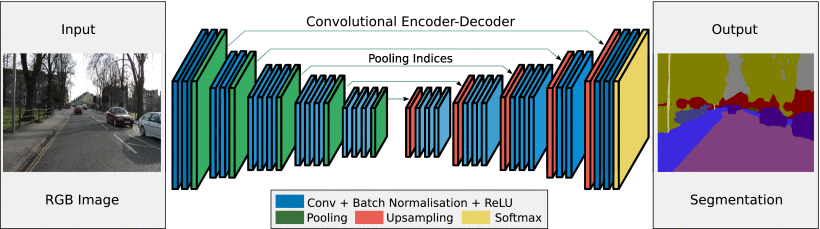
\includegraphics[width=\linewidth]{figures/chap223_segnet_arch.png}
	\caption[Encoder-Decoder-Architecture]{
		Encoder-Decoder-Architecture from SegNet. 
		On the left the encoder network, which reduces the size of the feature maps while processing. 
		On the right is the decoder network, which reconstructs the feature map to the size of the original input. 
		The yellow layer on the very right is the classification layer, here represented as softmax layer to create the output segmentation. 
		Copyright \copyright 2017 Creative Commons License. Reprinted by permission from \cite{Bad17-SegNet}.}
	\label{fig:ch2:sec2:encoder-decoder}
\end{figure}

\paragraph{Unpooling.}
The unpooling operation is the equivalent of the pooling operation.
Instead of reducing the size of feature maps $F^{n}_{c}$, they are enlarged.
As for pooling, no features are learned and there exist multiple methods to perform unpooling, two of them are illustrated in Figure \ref{fig:ch2:sec2:unpooling_1}.
Nevertheless, unpooling is not capable to fully reconstruct the information lost during the process of downsampling.
The result for \textit{bed of nails} are sparse feature maps $F^{n}_{c}$, while for \textit{nearest neighbor} the feature maps $F^{n}_{c}$ contain redundant information.
% In order to achieve a fine and detailed segmentation result, this is an interfering effect.
%For an architecture with max pooling and a mirrored structure of encoder and decoder network, this effect can be mitigated by saving the location of the maximal value during max pooling.
% In the following the unpooling result can be specified based on this information, as exemplified in Figure \ref{fig:ch2:sec2:unpooling_2} \cite{NHH15-DeConvNet} \cite{Fer19-SemSeg}.

% TODO recreate figure by myself with drawing program.
\begin{figure}
	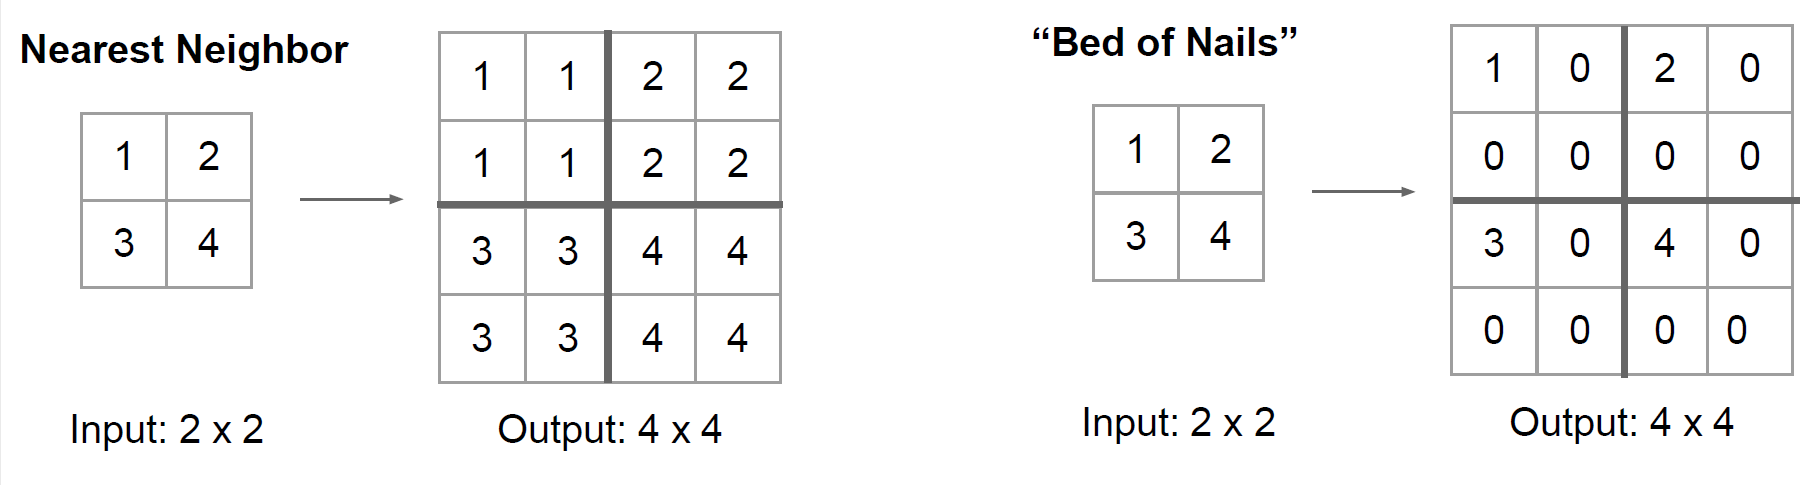
\includegraphics[width=\linewidth]{figures/chap223_unpooling1.png}
	\caption[Unpooling methods \textit{nearest neighbor} and \textit{bed of nails}]{
		Unpooling methods \textit{nearest neighbor} and \textit{bed of nails}.
		With \textit{nearest neighbor} enlarged feature maps are filled up with the same input value. 
		With \textit{bed of nails} sparse feature maps are created, that contain the input value filled up with zeros.
		\textit{TODO recreate figure with drawing program}}	
	\label{fig:ch2:sec2:unpooling_1}
\end{figure}
% \footref{fn:LJY10_StanfordLecture}
%	\footnotemark{\ref{footnote:LJY10_StanfordLecture}} 

% \begin{figure}
% 	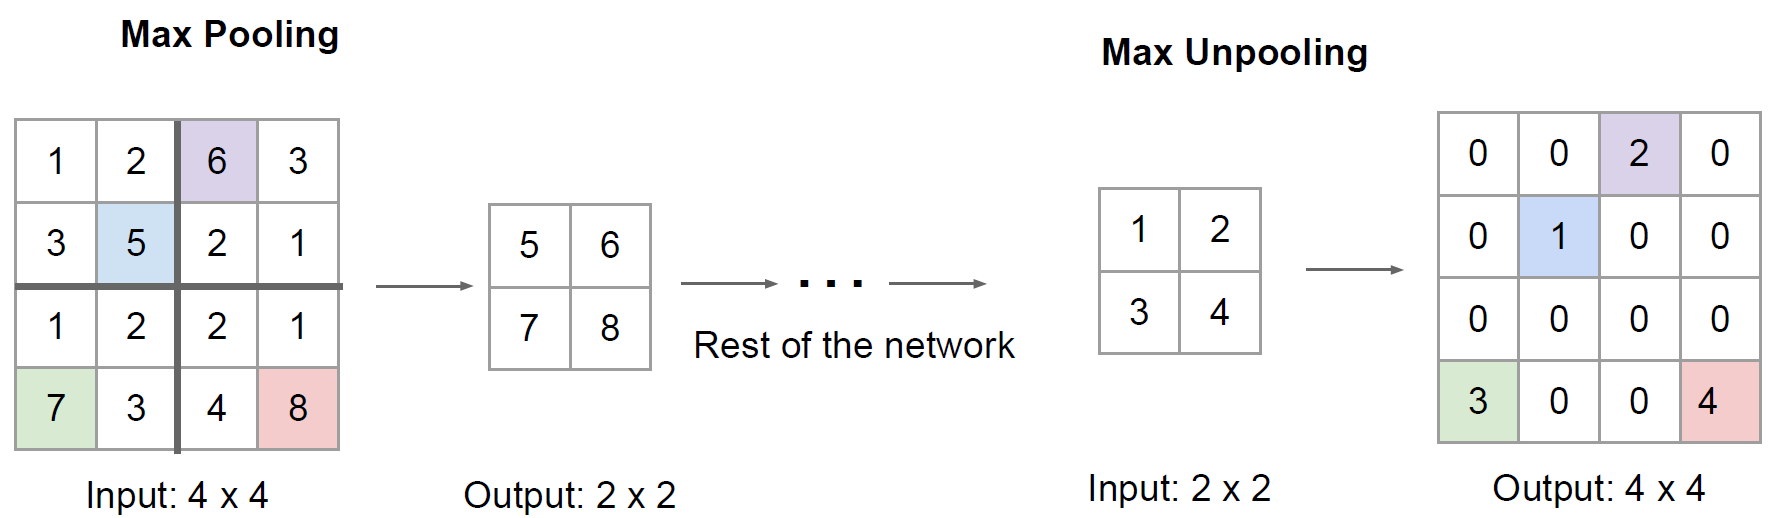
\includegraphics[width=\linewidth]{figures/chap223_unpooling2.png}
% 	\caption[Max Unpooling]{\textit{Max unpooling} \cite{Li17-StanfordLecture}. During max pooling the location of the maximal element is remembered. During max unpooling this location-information is reapplied to achieve a specified result, compared to the \textit{bed of nails} method.}
%	\label{fig:ch2:sec2:unpooling_2}
%\end{figure}

% We can observe that coarse-tofine object structures are reconstructed through the propagation in the deconvolutional layers; lower layers tend to capture overall coarse configuration of an object (e.g. location, shape and region), while more complex patterns are discovered in higher layers. 
% Note that unpooling and deconvolution play different roles for the construction of segmentation masks. Unpooling captures example-specific structures by tracing the original locations with strong activations back to image space. As a result, it effectively reconstructs the detailed structure of an object in finer resolutions. On the other hand, learned filters in deconvolutional layers tend to capture class-specific shapes. Through deconvolutions, the activations closely related to the target classes are amplified while noisy activations from other regions are suppressed effectively. By the combination of unpooling and deconvolution, our network generates accurate segmentation maps \cite{NHH15-DeConvNet}.

\paragraph{Transposed Convolution.}
As for pooling it is unpooling, the counterpart of convolution is transposed convolution.
Therefore, these operations also share common features and characteristics, like learnable filters or hyperparameters as \textit{kernel size}, \textit{padding} and \textit{stride}.
Transposed convolution can be used to enlarge feature maps or dense sparse feature maps, as created by the unpooling method "bed of nails".
% TODO clarify if Noh or Noh et al.
% Purpose of transposed conv for reconstruction.
In \cite{NHH15-DeConvNet} it is observed, that the lower layers of the decoder network handle coarse details (\eg location, shape and region), while the higher layers capture the fine and more complicated details.
This leads to a coarse-to-fine approach for the reconstruction through the decoder network.
In literature transposed convolution is also referred to as  \textit{deconvolution} \cite{NHH15-DeConvNet}, \textit{inverse convolution} \cite{Bad17-SegNet} or \textit{backwards convolution} \cite{LSD15-FCN}.
A visualization of transposed convolution is provided in \cite{DV19-ConvolutionGuide}.
% \footnote{F.-F. Li, J. Johnson and S. Yeung, 2018, "Stanford Lecture Detection and Segmentation": \url{http://cs231n.stanford.edu/slides/2018/cs231n_2018_lecture11.pdf}\label{fn:LJY10_StanfordLecture}}.

% TODO recreate figure by myself with drawing program.
\begin{figure}
	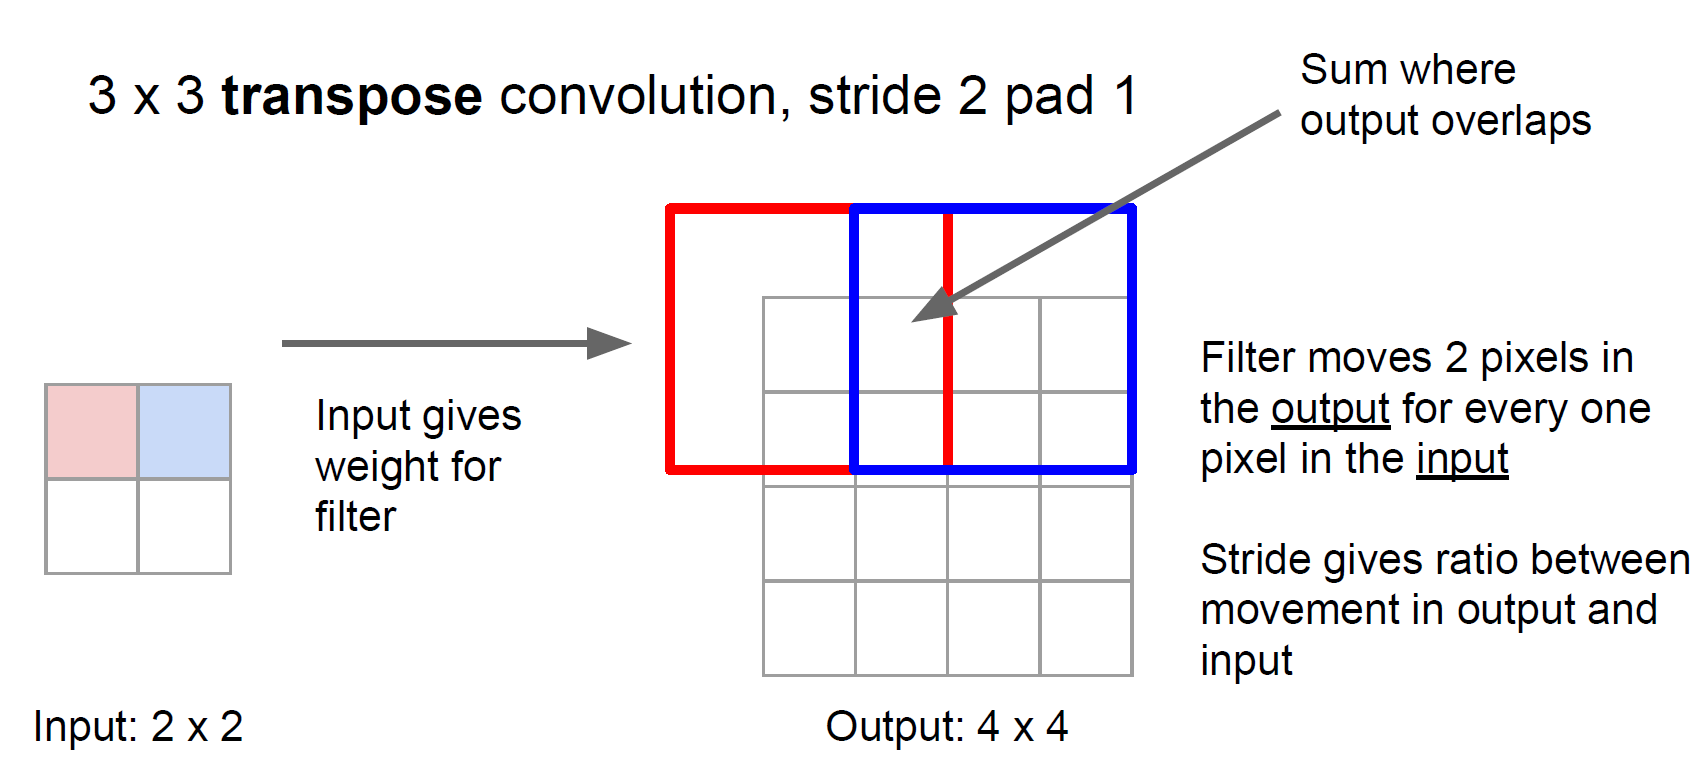
\includegraphics[width=\linewidth]{figures/chap223_transpose_conv.png}
	\caption[Transposed Convolution]{
		Example of the transposed convolution with $\textnormal{\textit{kernel size}} = 3 \times 3$, $stride = 2$ and $padding = 1$. 
		On the left is the input of size $2 \times 2$ \Unit{px} before the application of transposed convolution.
		On the right is the output of size $4 \times 4$ \Unit{px}. 
		The red and blue square visualize the application of the convolution kernel with $stride = 2$. 
		\textit{TODO recreate figure with drawing program}}
	\label{fig:ch2:sec2:transposed-conv}
\end{figure}


\subsubsection{Skip Connections} \label{ord:ch2:sec2:subsec_arch:skipconnections}

To resume the question of localization and enable detailed image reconstruction, skip connections are introduced. 
% This is due irretrievable loss of information during downsampling.
This concepts adverts from the idea of building a strictly sequential architecture.
Alternatively, skip connections are also named lateral or shortcut connections.
A skip connection is a link between two layers, which do not follow one after the other. 
The receiving layer may takes multiple inputs, one from the previous layer and another from the layer connected by the skip connection.
These inputs are combined in the depth by the concatenation operation, for this the inputs usually have the same spatial dimension.

Skip connections can be integrated in other architectures as \eg the encoder-decoder-architecture from \cite{RF15-U-Net} shown in Figure \ref{fig:ch2:sec2:unet}.
By doing so, layers that still contain localization information can be directly connected to layers that contain the developed classification information \cite{LSD15-FCN}.

\begin{figure}
	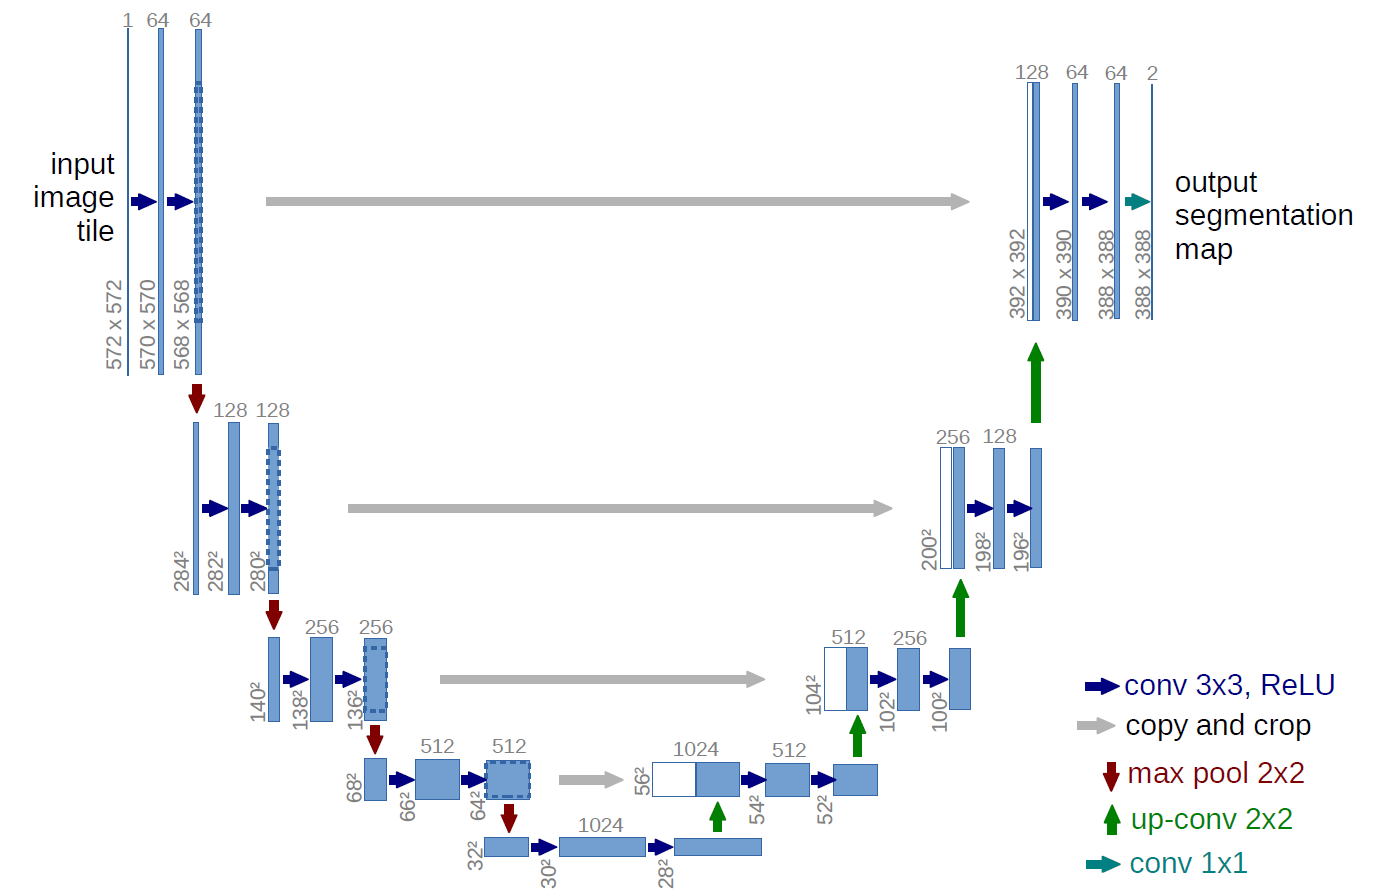
\includegraphics[width=\linewidth]{figures/chap223_unet.png}
	\caption[U-Net]{
		U-Net architecture. The left part of the shown network architecture represents the encoder network, while the right part represents the decoder network. 
		In between, the skip connections establish additional lateral links (visualized in gray) between the encoder and decoder network. 
		The skip connections exist on several levels to persistently combine classification and localization information. 
		Copyright \copyright 2015 Springer Nature. Reprinted by permission from \cite{RF15-U-Net}.}
	\label{fig:ch2:sec2:unet}
\end{figure}

In the following the effect of skip connections is exemplary demonstrated by the \gls{fcn} introduced in \cite{LSD15-FCN}.
The \gls{fcn} is based on the encoder-decoder-architecture with a relatively small decoder.
To compensate the absence of a deep decoder and refine the network, Long applies skip connections, that combine lower layers with the final prediction layer.
In order to compare the effect of skip connections, three models are created: one without skip-connection (\gls{fcn}-32s) and two with skip connection (\gls{fcn}-16s and \gls{fcn}-8s).
The number indicates the upsampling factor required from this point to the final predictions.
The \gls{fcn}-16s and \gls{fcn}-8s require less upsampling, due to their fusion with a lower layer.
\begin{figure}
	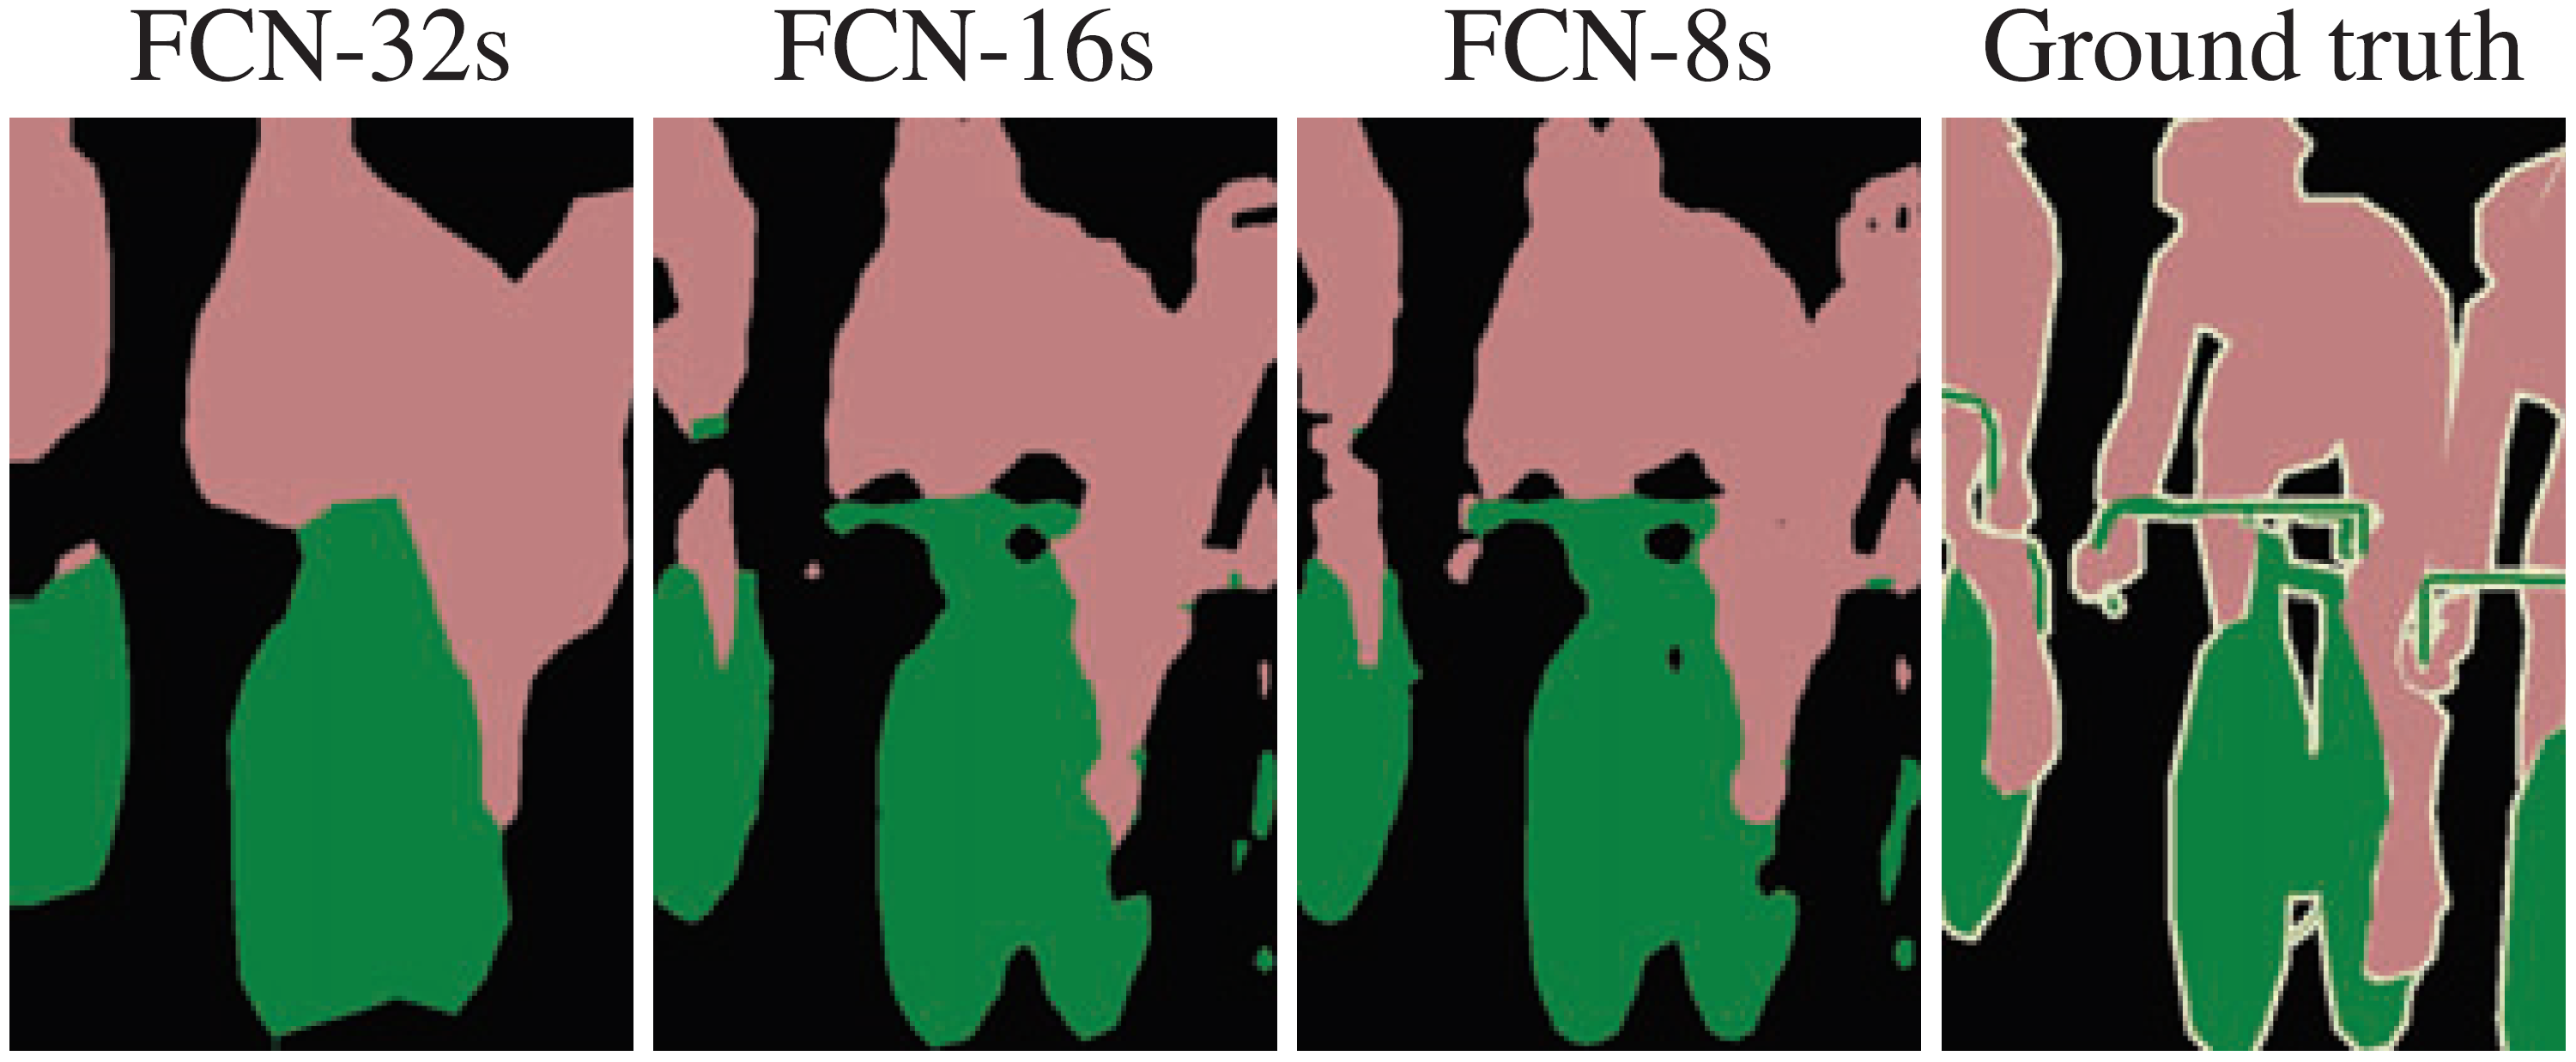
\includegraphics[width=\linewidth]{figures/chap223_fcn_results.png}	
	\caption[FCN Predictions]{
		Results of several variants of the \gls{fcn}. 
		It can be observed that the \gls{fcn}-32s creates a relatively coarse prediction compared to the networks with skip connections.
		In contrast the \gls{fcn}-8s achieves the best result with significantly improved level of detail and sharper borders.
		Copyright \copyright 2015 IEEE. Reprinted by permission from \cite{LSD15-FCN}.}
	\label{fig:ch2:sec2:fcn_res}
\end{figure}
The results shown in Figure \ref{fig:ch2:sec2:fcn_res} highlight the effect of skip connections in order to solve the question of localization.

\subsubsection{Pyramid Scene Parsing Network}

Another architectural component is introduced with the \gls{psp} network in \cite{Zhao17-PSP}.
% Problem / disadvantage of missing gobal context / subregions information
In this work it is stated, that the inclusion of more context information improves segmentation networks.
The quantity of the used context information is approximately indicated by the receptive field, which is size of the processed input region.
To enrich the context information it is proposed to combine the context information of several subregions.

This idea is based on \cite{He15-SPP}, where feature maps were processed by spatial pyramid pooling and thereby removed the limitations of fixed size.

% Idea: fused information from different subregions
To improve the context information, different subregions can be fused, similar as in 
% similar to \cite{He15-SPP} -> removes the fixed size contraint from CNNs

In \cite{Zhao17-PSP} this approach is further developed, by a hierarchical structure using multiple processing streams, also referred to as pyramid levels.
Each pyramid level processes the same feature map in various sizes.
Thereby, pooling layers with different filter sizes are applied to create feature maps of different sizes.
These feature maps are futher processed by convolutional layers and afterwards upsampled to a mutual size.
Last, the feature maps from the \gls{psp} module are concatenated with another and the features maps from the earlier processing step, as illustrated in Figure \ref{fig:ch2:sec2:psp}.
This \gls{psp} module enables the model to use more contextual information and therefore improve the segmentation result.
\begin{figure}
	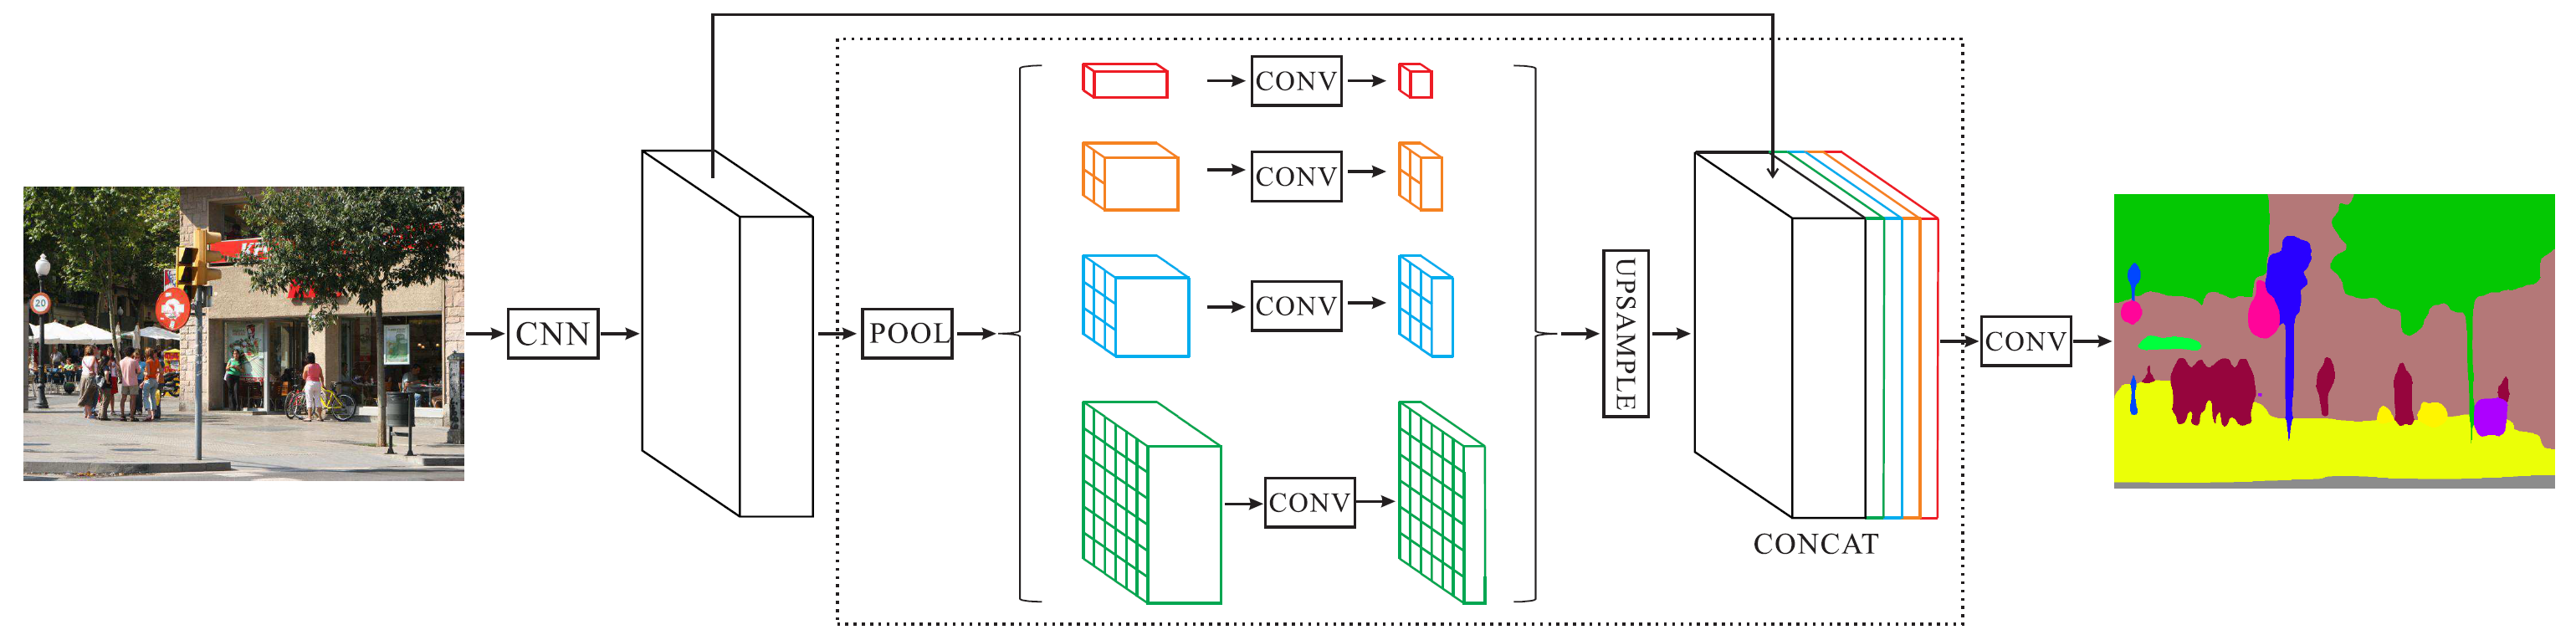
\includegraphics[width=\linewidth]{figures/chap223_psp.png}
	\caption[Pyramid Scene Parsing Network]{
		\gls{psp} Network with the pyramid pooling module in the middle.
		At (a) is the input image, which is fed into a \gls{cnn} for which a ResNet is used. 
		The feature maps (b) are the output of this \gls{cnn} and further processed in the pyramid pooling module (c).
		First, pooling with various sizes is applied, to create four feature maps of various sized, illustrated in different colors.
		These four feature maps are processed in the four pyramid level by convolutional layers.
		The respective sizes of the pyramid levels are $1 \times 1$, $2 \times 2$, $3 \times 3$ and  $6 \times 6$.
		The number of pyramid levels and their size can be modified.
		The results are upsampled to a mutual size and concatenated with another and the feature maps from (b).
		After the concatenation a final convolution is applied, which results in the final prediction (d) in the form of a segmentation map.
		Copyright \copyright 2015 IEEE. Reprinted by permission from \cite{Zhao17-PSP}.}
	\label{fig:ch2:sec2:psp}
\end{figure}



\subsubsection{DeepLab}
DeepLab is a \gls{dl} model for semantic segmentation developed by researchers from Google and first published in \cite{Chen16-DeepLab}.
It stands out due to the three techniques atrous convolution, \gls{aspp} \cite{He15-SPP} and, \gls{crf} \cite{KK12-CRF}, which are described in detail in \cite{Chen16-DeepLab}.
These techniques focus on the image's reconstruction in the upsampling process and therefore, improve the performance of the network.
A further development of these techniques is the DeepLabv3+ \cite{Chen18-DeepLab3+}, which set new performance records in 2018.

% \textbf{Atrous convolution} or dilated convolution modifies the kernel used for the convolution operation.	  The size of the kernel is extended and the upcoming gaps between the parameters are filled up with zeros.	The benefit is the coverage of a greater receptive field, without increasing the number of convolution parameters and so the computational load.
% \textbf{\gls{aspp}} is based on the concept of \gls{spp} introduced in \cite{He15-SPP}. 	\gls{spp} aims to combine images of different resolutions in order to obtain multi-scale information without increasing the computation time.	\gls{aspp} applies atrous convolution to the concept of \gls{spp}.	An input is fed into atrous convolution layers with different kernel sizes and the result is their combined output.
	
% \textbf{\gls{crf}} is statistical modeling method applied in \gls{ml}. \glspl{crf} aim to achieve sharper boundaries by considering the surrounding pixels before performing classification.		The functionality can be reviewed in detail in \cite{Chen16-DeepLab} and \cite{KK12-CRF}.	In contrast to most other segmentation models DeepLab does not use skip connections, but instead relies on \gls{crf} in order to recover fine details and the boundaries of objects to answer the question of localization.


\subsection{Data}\label{ord:ch2:sec2:subsec_data}
As image segmentation is a problem of supervised learning, a dataset with \gls{gt} is required.
For a dataset to be suitable in the field of \gls{dl} among others the following criteria should be met: size, quality and representation capability.
\begin{itemize}
	% Quantity data - size matters.
	\item The size of images within a dataset used for training a \gls{dl} model is crucial for its success.
	In general, small datasets, may not cover all vital characteristics to completely map a given objective.
	It has been shown in \cite{Banko01-ScalingData}, that the performance of networks can improve significantly using larger datasets for training.
	Also, in \cite{Halevy09-UnreasonableEffectivenessOfData} the effect of larger datasets is examined. 
	It is claimed that, using a larger dataset for training can improve the network's performance more than modifying the architecture of the network \cite{Ger17-HandsOn}.
	This highlights the importance of datasets with sufficient quantity to increase the performance of networks.
	% Quality data.
	\item The quality of the training data has a high impact on the model performance as well.
	Data, that is inconsistent, incomplete, erroneous, or too noisy, can lead to a significant decrease in performance \cite{Gudivada2017-DataQuality}.
	Training with poor quality data makes it more difficult for a model to detect and understand the elemental features and patterns, that are required by a model to perform well \cite{Ger17-HandsOn}.
	% TODO affect of poor quality data for object detection or segmentation segmentation. "With respect to the task of segmentation segmentation correctness is very significant, for the accuracy of the edges is crucial if a pixel is labelled with the correct class or not."	
	% Representative data.
	\item The capability of dataset to represent a given problem is another elemental characteristic.
	To enable a model to generalize and perform well, it is essential for the training data to be representative for the problem \cite{Ger17-HandsOn}.
	Goodfellow \etal also states, that the performance of a \gls{dl} model is strongly connected to the representation of the data \cite{Goodfellow-et-al-2016}.
	The best approach to do so, is to include samples of this specific problem or of samples from the same domain.	
	
	If the given problem is not represented within the samples of the used datasets, this may cause a decrease in performance.
	This may happen if a specific problem should be solved by a model, that is trained on general 'all-use-datasets', like PASCAL \gls{voc} \cite{Eve20-PascalVOC}, COCO \cite{Lin14-Coco} or ImageNet \cite{Deng09-ImageNet}.
	Therefore, it is important to pay attention to representation capability of the used dataset.
	% TODO \cite{Xu16-InteractiveObjectSelection}  The performance is evaluated on MS COCO with seen and unseen categories. Two points can be seen here: 	1. The significant drop in IU (Intersection over Union) from seen to unseen categories.  2. This network using user interaction suffers a way smaller drop in IU.
	%	For example, the aim of a DL model may be to detect a certain manufacturing part from an industrial scope.
	%	But without a dataset that represents this problem well enough, by containing samples from industrial scopes, the performance of the DL model may be significantly worse.
	%	This may results in a decrease of performance, because the capabilities of \gls{dl} models are strongly connected with the representation of the data \cite{Goodfellow-et-al-2016}.
\end{itemize} 
% Very hard and expensive to obtain data for segmentation and special domains.
It is a challenge to obtain a dataset, that meets these criteria.
The acquisition of new image datasets is very expensive in time and cost.
Datasets for semantic segmentation are even more expensive due to the high effort required to label images on pixel-level.
Especially, uncommon or confidential domains (\eg medical or industrial domains) are rarely covered in public datasets.
For example, the manufacturing process in a closed industrial environment may contain unique objects or uncommon surroundings, that are hardly ever represented in large-scale, open source datasets.

% New ways to obtain GT -> Labeltool, Interactive methods, AI-Simulation 
New approaches have been created, to facilitate the process of creating new dataset and label images with pixel-level accuracy.
An efficient and common way is a program, that simplifies labeling process by providing an user interface and multiple methods to create and save label.

Specific \textit{label} or \textit{annotation tools} provide a user interface and easy-to-use methods to create and edit labels. 
Due to the hight demand for labeled training data there are various labeltools available.\footnote{E. Cerna, \textit{Image Annotation Tools: Which One to Pick in 2020?} \url{https://bohemian.ai/blog/image-annotation-tools-which-one-pick-2020/}}
To simplify the manual process of labeling for a human user interactive methods facilitate the label process (see Chapter \ref{ord:ch2:sec3}).
Another approach is to create synthetic datasets like the SYNTHIA dataset \cite{Zol19-Temporal} and use them for training of semantic segmentation networks \cite{Chen18-SyntheticData}.


\subsection{State-of-the-art}\label{ord:ch2:sec2:subsec_compare}

An overview about the performance of previously introduced and current state-of-the-art networks is given in Table \ref{tab:ch2:stae-of-the-art}.
As benchmark dataset the PASCAL \gls{voc} test set \cite{Eve20-PascalVOC} and as metric the \gls{miou} were selected, due to their widespread usage.
Notable is the rapid increase of performance over the last years, which emphasizes the relevance and research interest on this field of study.
The model delivering the best performance is currently the EfficientNet introduced in \cite{Zoph20-EfficientNet}, which is superior due to the application of so-called \textit{self-training}.
\begin{table}[h!]
	\centering
	\begin{tabular}{l|r|r}
		\textbf{Model} 								&  \textbf{\gls{miou}}\\
		\hline
		\gls{fcn}-8s \cite{LSD15-FCN} 				& 62.2\\
		DeconvNet \cite{NHH15-DeConvNet}			& 72.5\\
		DeepLab-CRF \Cite{Chen16-DeepLab} 			& 79.7\\
		\gls{psp}Net \cite{Zhao17-PSP}				& 85.4\\
		DeepLabv3+ \cite{Chen18-DeepLab3+} 			& 87.8\\
		EfficientNet \cite{Zoph20-EfficientNet} 	& 90.5\\
	\end{tabular}
	\caption[Comparison of image segmentation models]{
		Comparison of image segmentation models on the PASCAL \gls{voc} 2012 test set. 
		An more detailed overview with all officially submitted models can be reviewed PASCAL \gls{voc} 2012 leaderboard.\footnotemark 
	}
	\label{tab:ch2:stae-of-the-art}
\end{table}
\footnotetext{Segmentation Results: Leaderboard PASCAL \gls{voc} 2012: \url{http://host.robots.ox.ac.uk:8080/leaderboard/displaylb_main.php?challengeid=11&compid=6}}
%TODO ensure the footnote is on the same page as the table
% !TeX root = ../../main.tex
% Add the above to each chapter to make compiling the PDF easier in some editors.

\section{Interactive Segmentation}\label{ord:ch2:sec3}

Image segmentation takes as input $\textbf{x}$ only the image itself.
In contrast interactive segmentation takes beside the image some additional information interactively provided by an user.
% Interactive segmentation segmentation takes advantage of additional information interactively provided by an user.
This additional information is especially beneficial, because it is manually picked by the valuable image processing capabilities of a human users.
Due to this, interactive segmentation networks are provided with high level guidance on the object of interest.
Depending on the type of interaction, the receipt of the user input may be more or less elaborately, which leads to a fundamental difficulty of interactive methods in general.
User interaction is considered to be expensive and elaborate.
% Especially, for deep learning tasks a great quantity of images is required.

The interactive segmentation of an instance may be interpreted as semantic segmentation with two classes: the foreground object to segment and the background.
In order to segment multiple objects in an image, multiple applications of these interactive methods are required.
% TODO scope of interactive segmentation here, the class is assigned manually?
In the following the principles of interactive segmentation concepts are introduced, on which the methods used in the benchmark study are built on.

\subsection{Classical Concepts}\label{ord:ch2:sec3:subsec1}
Before the upcomming of \gls{dl} and \glspl{cnn}, segmentation was already performed with classical image processing.
These methods also focus on the extraction of a foreground object from the background by little user interaction.

% GraphCut and GrabCut
Prominent algorithms are Graph Cut \cite{BJ01-GraphCut} and GrabCut \cite{RKB04-GrabCut}.
As user interaction GrabCut requires a loose bounding box and optionally defining explicit image parts as fore- or background.
%Everything outside the bounding box and the borders itself are defined as background, while the inside of the box is segmented based on contrast and color information.
%Further, the goodness of the result may be enhanced by iteratively defining explicit image parts as fore- or background.

% Watershed
Another still relevant method to perform instance segmentation is the watershed transformation \cite{VS91-Watershed}.
This method interactively collects fore- and background markers from an user in order to perform segmentation.
The watershed method is part of the benchmark study and elaborately examined in Section \ref{ord:ch3:sec2}.

% Superpixels
Last, an algorithm using so-called \textit{Superpixel} was introduced in 2003 \cite{RM03-Superpixel}.
Superpixels are groups of connected pixels, that share similarities in color or low-level features as contour, brightness or texture.
Further, these Superpixels are used to perform segmentation.
This algorithms is still a current research topic, an overview of several state-of-the-ar approaches is given in \cite{SHL16-SuperpixelEvaluation}.
 
% Final tought
Although, these algorithms are based on classical image processing, they remain relevant in modern problem and research topics.
%These classical methods may perform very well on certain images, but tend to reach their limitations as they deal with more complex structures.
%They are often outperformed on current benchmark datasets by more recent \gls{dl} methods.
% This is due to their rather simple processing of superficial characteristics \eg edges, textures, contrast and color.
% On the contrary \gls{dl} based methods are capable to examine images on a deeper level and so understand more complicated structures.


\subsection{\gls{dl} User Point Concepts}\label{ord:ch2:sec3:subsec2}

\subsubsection{Basic Concept}
% DL focus 
Mordern interactive segmentation algorithms combine \gls{dl} models and additional user input.
As \gls{dl} models usually \glspl{cnn} for image segmentation are applied.
% Obtaining points on fore- and background
User point centered concepts obtain the user input in the form of clicks on the image.
The user clicks are often differentiated between clicks on the foreground object and clicks on the background.
The input $\textbf{x}$ of an interactive segmentation network is a combination of the image and the user clicks.

% TODO probability map
This fundamental concept is used for various interactive segmentation models \cite{Xu16-InteractiveObjectSelection} \cite{MVL18-ITIS} and exemplary shown in Figure \ref{fig:ch2:sec3:ifcn}
% IOG and DEXTR explained in detail in following chapter.
Further, the methods \gls{dextr}  \cite{Man18-DEXTR} and \gls{iog} \cite{Zha20-IOG} also follow a user point centered concept. They are part of the benchmark study and extensively described in Section \ref{ord:ch3:sec3} and \ref{ord:ch3:sec4}.
\begin{figure}
	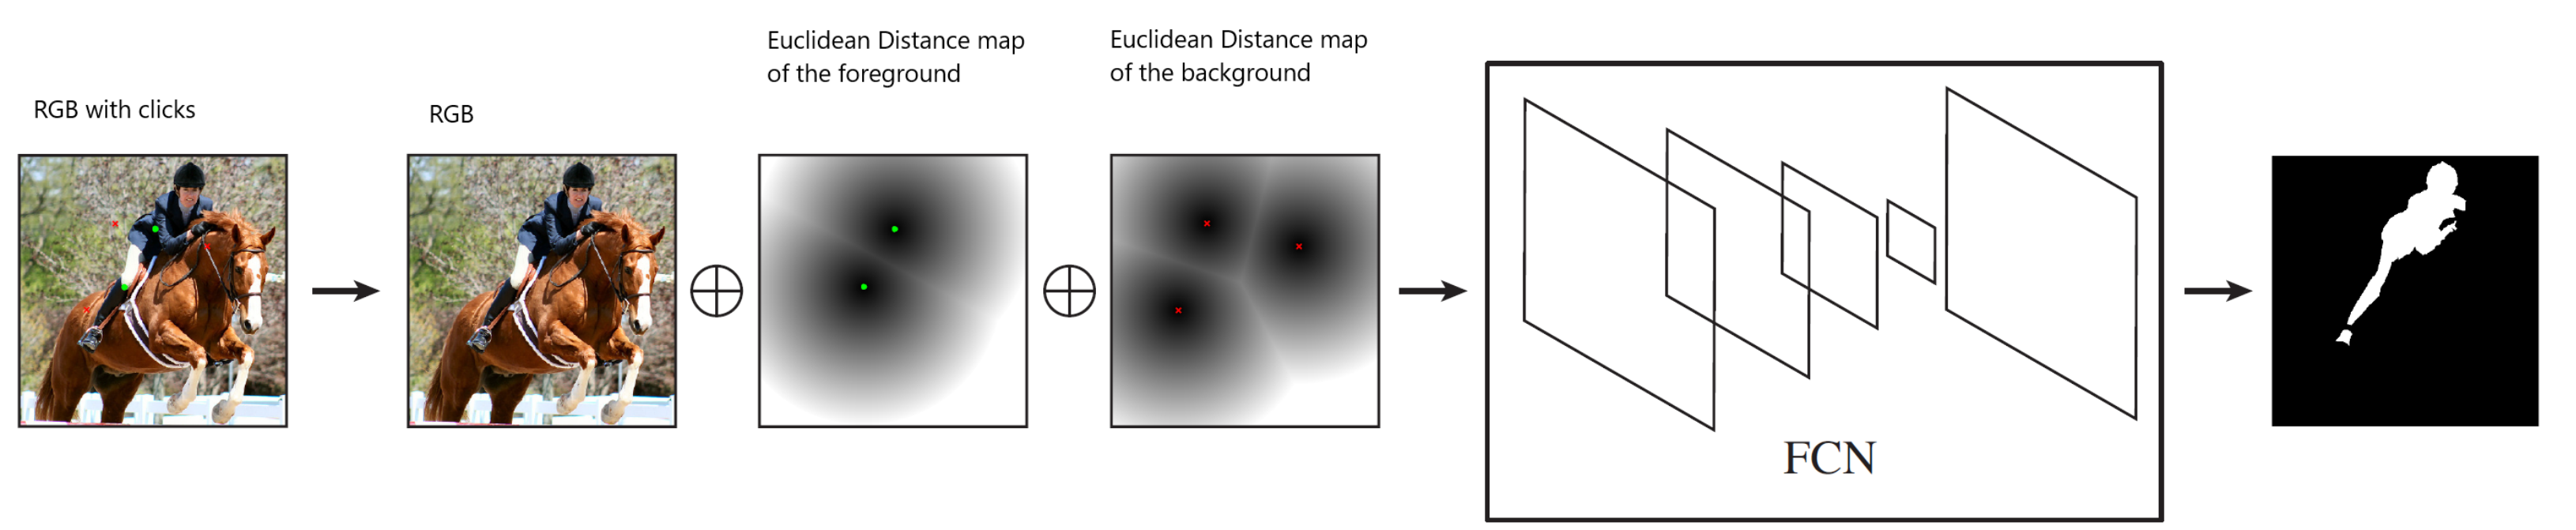
\includegraphics[width=\linewidth]{figures/chap232_ifcn.png}
	\caption[Interactively Fully Convolutional Network]{
		Illustration of the pipeline from the \gls{ifcn}.
		The input is a \gls{rgb} image with user clicks.
		This input is displayed in its individual parts as \gls{rgb}, map of the fore- and background points.
		The network in use is based on the \gls{fcn} and outputs a binary segmentation result.
		Copyright \copyright 2016 IEEE. Reprinted by permission from \cite{Xu16-InteractiveObjectSelection}
	}\label{fig:ch2:sec3:ifcn}
\end{figure}

\subsubsection{Representation of User Clicks and Model Input}
The user clicks are converted to points and mapped into new heatmaps, that have the same spacial dimension as the input image.
In order to distinguish between fore- and background points, there exist separate heatmaps for fore- and background.
In some literature the foreground points are also called \textit{positive} points, while the background points are called \textit{negative} points.
If there is are only one type of points, there also exist only one heatmap.

% Modification of points -> gauss or euclidean
The heatmaps are further processed, in order to highlight the set user points.
This may be achieved by the conversion into an Euclidean distance map \cite{Dan80-EuclideanDistanceMapping} (see Figure \ref{fig:ch2:sec3:ifcn}) or the application of a Gauss filter.
% TODO source or footnote for Gauss filter

% 3 RGB Channels + 2 Heatmaps = 5-Channel input
The image is usually colored with the three \gls{rgb} channels.
The heatmaps have the same size as the image and are appended to the image as additional channels.
%This results in a five- or four-channel input for the interactive segmentation network, depending on the number of heatmaps.
This results in a five-channel input using fore-and background heatmaps or in a four-channel input using just a foreground heatmap.

The processed points on the heatmaps and the user clicks on the image are located exactly at the same position on different channels.
This matching is vital for the functionality of the segmentation method.
The user points provide high level guidance for the network to enhance the location and differentiation of fore- and background.
The multidimensional input functions as model input $\textbf{x}$ for the semantic segmentation network.

Interactive segmentation networks are often based on normal segmentation networks, \eg the \gls{fcn} in the \gls{ifcn} \cite{Xu16-InteractiveObjectSelection} or the DeepLabv3+ in the \gls{itis} network \cite{MVL18-ITIS}.
As for segmentation networks, the prediction $\hat{y}$ of interactive networks is a probability map.

\subsubsection{Interactive Refinement}
A fundamental advantage of interactive methods is the presence of a human user.
The interactive segmentation network may not always deliver a satisfactory result in the initial execution.
For this case, interactive methods often provide the option to refine the initial result.
In order to apply refinement, the user sets an additional click on the fore- or background region, where the segmentation fails.
This refinement click is added to the corresponding heatmap and the network is executed again based on the updated input.
This refinement process may be applied iteratively by the user.

With refinement the user provided guidance is additionally reinforced.
Further, interactive refinement specifically focuses on regions of failure, while other models without user interaction must rely on their initial predictions.


\subsubsection{Characteristics}
% Similar to normal segmentation networks.
Interactive segmentation networks almost have the same characteristics as normal segmentation networks.
For training they require the multidimensional input $\textbf{x}$, while the label $y$ remains the same.
% Simulation of user clicks.
To create suitable input $\textbf{x}$, user clicks are regularly simulated.
The simulation of the user clicks is based on the corresponding \gls{gt}.
On the one hand, the application of simulation has certain advantages, compared to manually acquiring user clicks.
Simulations are easily scalable, faster and cheaper than the acquisition of manual clicks from real users.
% Second, in a simulation no variance occurs between the set clicks of various users, if the .
% TODO is this necesarrily an advantag?
% Third, simulations have the possibility to effortless create various click patterns, that \eg vary the set click by a random offset, in order to simulate a various types of user behavior.
On the other hand, simulations are only capable to replicate the user's behavior to a certain extent.
Further, the involvement of human users is especially important for methods, which performance depends on user interactions.


% Refinement Training
The training setup for iterative refinement is more elaborate.
The refinement clicks are simulated online during the training process.
In the simulation the refinement clicks are usually set on the greatest error, which is calculated based on the \gls{gt} and the prediction $\hat{y}$ of the previous model execution.

\subsubsection{Variations}
% Special Methods 
%    - Iterative learning
%    - Fusion networks
While the presented concepts is the most common approach and achieves state-of-the-art results, there are other mention-able ideas and variations:
\begin{itemize}
	% One click
	\item \textbf{One-Click Segmentation} is introduced in \cite{Maj20-One-Click} and this networks requires only one click one foreground click.
	This click is processed as foreground click and enforced with a Gauss filter.
	The segmentation is based on the DeepLab network.
	Despite the user interaction is most simple, this approach can not compete with the performance of state-of-the-art networks.
	
	\item The \textbf{\gls{fctsfn}} stands out, due to the separate processing of image and user clicks \cite{Hu19-TwoStreamFusionNetwork}.
	% The fore- and background points are converted into two feature maps, that contain an Euclidean distance map.
	The user clicks and the image are processed separately by two streams.
	These two processing streams share the same architecture based on VGG16, but have their own weights.
	The intent is to learn the deep features from image and user clicks individually.
	Further, the two streams are combined and processed together to create one prediction.
	
	\item \textbf{Iterative training} is applied in the \gls{itis} network \cite{MVL18-ITIS}.
	Every epoch a new refinement click is added to the multidimensional input.
	This click is simulated during the training process, based on the classification result of the previous epoch.
	It is claimed, that this novel \textit{iterative training procedure} significantly improves the networks performance.
	
\end{itemize}


\subsubsection{Evaluation and State-of-the-Art Networks} \label{ch2:sec3:eval_interactive_methods}
% Describe Evaluation metrics: clicks requried for certain iou and iou at certain amount of clicks
For a reliable evaluation of interactive methods the user interaction has to be taken into account.
For user interactions based on clicks, two metrics are widely used together, represented in Table \ref{tab:ch2:interactive-stae-of-the-art}. 
The first metric lists the number or clicks, that a model requires to reach a certain level of performance. 
The number of clicks must not be even, due to the averaging of all results of the dataset.
The second metric lists the models performance for a certain amount of clicks.

% Limitations.
Yet, with these metrics, a uniform evaluation reaches some limitations, addressed in the following:
The first metric is actually only applicable if a method has the possibility to perform refinement.
The second metric does not always enable a fair comparison, because for various methods the underlying functioning may be different. 
For example, the minimal required amount of clicks may be lower or higher than the amount of clicks, which is set for comparison.

% Problems with the evaluation of time.
In terms of interactive methods, the time required for the user interaction is fundamental for the evaluation.
The measured time by single papers is not comparable, due to the missing of a common setup to perform uniform user studies for these novel methods.
With these metrics the time is only approximated by the number of clicks.
But there are no indicators, that describes how elaborate it is and how much time it needs to set these clicks.
Further, there is no common metric to evaluate the usability of these interactive methods

Nevertheless, these metrics are the current state to evaluate interactive segmentation methods.
They are still suitable to meaningful compare interactive segmentation models, but their limitations have to be noted.
A comparison of several mentioned methods and the current state-of-the-art methods is given in Table \ref{tab:ch2:interactive-stae-of-the-art}.


% State of the art
\begin{table}[h!]
	\centering
	\begin{tabular}{l|c|c}
		\textbf{Model} & \textbf{Number of clicks} & \textbf{\gls{iou} (\%) @ 4 clicks} \\
		& PASCAL \gls{voc} @85\% & PASCAL \gls{voc} \\
		\hline
		% TODO add watersheds if available for PASCAL VOC
		Graph Cut \cite{BJ01-GraphCut}									  & > 20 & 41.1\\
		\glsentryshort{ifcn} \cite{Xu16-InteractiveObjectSelection}       & 6.9  & 75.2\\
		\glsentryshort{risnet} \cite{Liew17-RegionalInteractiveImageSeg}  & 5.7  & 80.7\\
		\glsentryshort{itis} \cite{MVL18-ITIS}			 				  & 3.4  & -\\
		\glsentryshort{fctsfn} \cite{Hu19-TwoStreamFusionNetwork}		  & 4.6  & -\\
	    \glsentryshort{dextr} \cite{Man18-DEXTR} 	     				  & 4    & 91.5\\
		\glsentryshort{iog} \cite{Zha20-IOG}	 	    				  & 3    & 94.4\\
	\end{tabular}
	\caption[Comparison of interactive segmentation models.]{
		Comparison of interactive segmentation models on the PASCAL \gls{voc} 2012 test set.
		It can be seen, that interactive segmentation methods have developed quickly. 
		They strongly improved in terms of required clicks and \gls{iou}.
		% TODO ?? PASCAL \gls{voc} is at its limit to be suitable to evaluate semantic segmentation.
	}
	\label{tab:ch2:interactive-stae-of-the-art}
\end{table}

\subsection{\gls{dl} Polygon Concepts}\label{ord:ch2:sec3:subsec3}
This concept is based on the idea to use a \gls{dl} model to predict a polygon.
The polygon represents the segmentation mask and within the desired object.

The following is a brief summary of the method represented in \cite{Ling19-Curve-GCN}.
% Workflow + UI
As initial user interaction a loose bounding box around the object of interest is required.
Based on this box the image is cropped and the crop is used as model input.

% Architecture
The \gls{dl} model consists out of a combination of several subnetworks and architectural components.
First, a \gls{cnn} takes the cropped image as input and performs as encoder.
This encoder provides the extracted features and a boundary prediction to the third component.
Second, a fixed size polygon is initialized, to transform the task into a graph problem.
Third, a multi-layer \gls{gcn} iteratively shifts the position of each polygon node towards the object boundary. 
This method is named \textit{Curve-\gls{gcn}}, inspired by the \textit{curved} approximation of a closed polygon.
% Good user interaction - refinement
The user is able to perform refinement, by interactively moving single nodes of the polygon.
% Performance
% The performance of the \textit{Curve-\gls{gcn}} is only represented on the Cityscapes Dataset, but it claim to perform 
Details of this method can be reviewed in \cite{Ling19-Curve-GCN}.
In experiments on datasets as CityScapes or Rooftop the \textit{Curve-\gls{gcn}} is outperformed by the \gls{iog} methods, which is presented in \ref{ord:ch3:sec4}.

% Vorreiter von Curve GCN \cite{Acu18-Polygon-RNN++}
The predecessor of the \textit{Curve-\gls{gcn}} is based on \glspl{rnn} and introduced in \cite{Acu18-Polygon-RNN++}.






% !TeX root = ../../main.tex
% Add the above to each chapter to make compiling the PDF easier in some editors.

\chapter{Benchmark Methods}\label{ord:ch3}

In this chapter the interactive methods used in the benchmark study are introduced.
Their technical functionality is explained in detail, while the motivation behind their selection is discussed in Section \ref{ord:ch4:sec2}.

The following methods all perform in the same setup: An image, that contains one or multiple objects, is shown to the user and the user's task is to create separate masks for the objects in the image.
To segment multiple objects in one image, the method has to be applied for each object separately.
The images are usually colored and contain the three color channels \gls{rgb}.
%TODO what about gray scale images
%TODO class-agnostic image segmentation

% !TeX root = ../../main.tex
% Add the above to each chapter to make compiling the PDF easier in some editors.

\section{Polygon Drawing}\label{ord:ch3:sec1}

In contrast to previously introduced methods, this polygon drawing proceeds manual.
By manually setting points on the object in the image a polygon is created.
From three points a polygon is spanned, where each point functions as a node.
% Each point has two edges.
The area inside the polygon represents the object mask.
In order to create a suitable mask the points should be set on the boundary of the desired object.

There are two ways to set points.
First, to set one point after another by one mouse click for each point.
Second, to draw multiple points by moving the mouse, this also referred to as \textit{stroking}.
In detail this is done, pressing the left mouse button, moving the mouse and releasing the left mouse button.
On the drawn way multiple points with a certain spacing are set.

Further, there are additional features implemented, in order to facilitate the drawing process.
Each new set point is automatically included into the polygon's nearest edge.
Set points can be relocated by a functionality similar to \textit{drag and drop}.
A set point can be removed by uniting it with another point and thereby only one point remains.


% !TeX root = ../../main.tex
% Add the above to each chapter to make compiling the PDF easier in some editors.

\section{Extreme Points}\label{ord:ch3:sec2}
Citation test~\parencite{latex} \cite{Zha2020}.

\subsection{Subsection}\label{ord:ch3:sec2:subsec1}

See~\autoref{tab:ch3:sample}, \autoref{fig:ch3:sample-drawing}, \autoref{fig:ch3:sample-plot}, \autoref{fig:ch3:sample-listing}.

\begin{table}[htpb]
  \caption[Example table]{An example for a simple table.}\label{tab:ch3:sample}
  \centering
  \begin{tabular}{l l l l}
    \toprule
      A & B & C & D \\
    \midrule
      1 & 2 & 1 & 2 \\
      2 & 3 & 2 & 3 \\
    \bottomrule
  \end{tabular}
\end{table}

\begin{figure}[htpb]
  \centering
  % This should probably go into a file in figures/
  \begin{tikzpicture}[node distance=3cm]
    \node (R0) {$R_1$};
    \node (R1) [right of=R0] {$R_2$};
    \node (R2) [below of=R1] {$R_4$};
    \node (R3) [below of=R0] {$R_3$};
    \node (R4) [right of=R1] {$R_5$};

    \path[every node]
      (R0) edge (R1)
      (R0) edge (R3)
      (R3) edge (R2)
      (R2) edge (R1)
      (R1) edge (R4);
  \end{tikzpicture}
  \caption[Example drawing]{An example for a simple drawing.}\label{fig:ch3:sample-drawing}
\end{figure}

\begin{figure}[htpb]
  \centering

  \pgfplotstableset{col sep=&, row sep=\\}
  % This should probably go into a file in data/
  \pgfplotstableread{
    a & b    \\
    1 & 1000 \\
    2 & 1500 \\
    3 & 1600 \\
  }\exampleA
  \pgfplotstableread{
    a & b    \\
    1 & 1200 \\
    2 & 800 \\
    3 & 1400 \\
  }\exampleB
  % This should probably go into a file in figures/
  \begin{tikzpicture}
    \begin{axis}[
        ymin=0,
        legend style={legend pos=south east},
        grid,
        thick,
        ylabel=Y,
        xlabel=X
      ]
      \addplot table[x=a, y=b]{\exampleA};
      \addlegendentry{Example A};
      \addplot table[x=a, y=b]{\exampleB};
      \addlegendentry{Example B};
    \end{axis}
  \end{tikzpicture}
  \caption[Example plot]{An example for a simple plot.}\label{fig:ch3:sample-plot}
\end{figure}

\begin{figure}[htpb]
  \centering
  \begin{tabular}{c}
  \begin{lstlisting}[language=SQL]
    SELECT * FROM tbl WHERE tbl.str = "str"
  \end{lstlisting}
  \end{tabular}
  \caption[Example listing]{An example for a source code listing.}\label{fig:ch3:sample-listing}
\end{figure}

% !TeX root = ../../main.tex
% Add the above to each chapter to make compiling the PDF easier in some editors.

\section{Deep Extreme Cut}\label{ord:ch3:sec3}

In \cite{Man18-DEXTR} the \gls{dextr} method for interactive segmentation is introduced.
This method follows a user point centered approach based on \gls{dl}, as introduced in Subsection \ref{ord:ch2:sec3:subsec2}.

\subsection{Method Description}\label{ord:ch3:sec3:subsec1}

% Workflow
The required user interaction are four clicks in the form of extreme points.
These points are the right-most, left-most, bottom and top pixels of an object, illustrated in Figure \ref{fig:ch3:sec3:user_interaction}.
They represent the most extreme pixels and therefore, are referred to as extreme points.
The obtained user clicks are further processed and the \gls{dl} model predicts an object mask.

% Advantage over other methods
Extreme points provide a valuable guidance for the segmentation network.
First, a bounding box can easily be derived from them.
Second, extreme points are naturally located at the boundary of the object.
This provides the network with high level guidance on the localization of the boundary.
% In the upsampling process this becomes especially useful, in order to reconstruct sharper borders.
With reference to the information content, extreme points are more valuable than a bounding box.

\subsection{Model Input and Representation of User Clicks}\label{ord:ch3:sec3:subsec2}

The creation of the model input $\textbf{x}$ may be separated into three processing steps.

% Crop image based on bbox
First, the image is preprocessed. 
A bounding box is derived from the extreme points. 
This bounding box is enlarged by $p_{{box}}$ \Unit{px}, to include context from the surrounding region.
% Zero Padding
If the enlarged bounding box extends over the original image boundary, the intensity values of the pixels outside the image domain are set to zero.
Manisis \etal refers to this treatment as \textit{zero padding} \cite{Man18-DEXTR}, which is illustrated at the bottom of Figure \ref{fig:ch3:sec3:user_interaction} and \ref{fig:ch3:sec3:rgb_channel}.
In order to focus on the object of interest, the image is cropped based on the enlarged bounding box.
The image crop is resized to the size of $512 \times 512$ \Unit{px}, to create inputs of constant size for the segmentation network.

\begin{figure}
	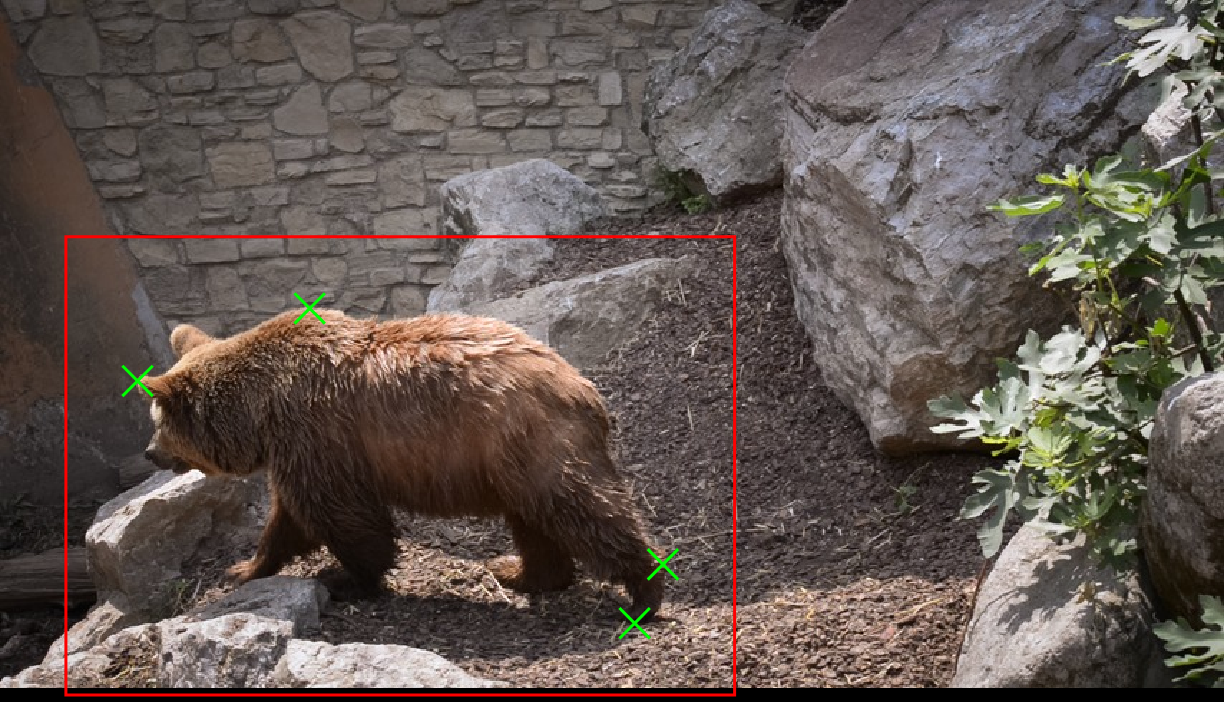
\includegraphics[width=\linewidth]{figures/chap33_bear_bbox.png}
	\caption[DEXTR User Interaction]{		
		Image with the obtained user input for the \gls{dextr} method and the first processing step.
		The extreme points are visualized as green crosses.
		The bounding box is enlarged by $p_{{box}} = 50$ \Unit{px}, shown in red.
		The enlarged bounding box extends the image boundary, therefore \textit{zero padding} is applied.
		The corresponding cropped and resized image is shown in Figure \ref{fig:ch3:sec3:rgb_channel}.
	}
	\label{fig:ch3:sec3:user_interaction}
\end{figure}


% One feature map with extreme points
Second, the four extreme points are converted into one heatmap.
The points in this heatmap are located on the boundary of the object.

To highlight the extreme points a 2D Gaussian is centered around each point $ \textbf{p} (x_p, y_p) $ with the another points $ \mathbf{x} = (x, y) $ by
% Impelemtation in HDevelop:
% ResGauss := exp(-4 \cdot log(2) $\cdot$ ((Rows-PointRow)*(Rows-PointRow) + (Cols-PointCol)*(Cols-PointCol)) / (GaussSigma * GaussSigma))
\begin{equation} \label{equ:gauss}
	\centering
	Gauss \left( x,y \right)  = max \left( g\left( x,y\right) , \frac{\exp(- 4 \log_{2}(| \textbf{x} - \textbf{p} |_2)}{\sigma^{2}}\right) 
\end{equation}
where $ g (x,y) $ is the current grayvalue of the heatmap at position $ (x, y) $ and $ \sigma = 10 $ representing the standard deviation of the Gauss filter.
This heatmap is vital for the method, because of the high level guidance for the deep segmentation network.
A closeup of a point centered by the 2D Gaussian is visualized in Figure \ref{fig:ch3:sec3:gauss_centered_point}.

Third, the heatmap has the size of $512 \times 512$ \Unit{px} and is concatenated with the RGB image.
This results in the four-channel \gls{dextr} model input, which is illustrated in Figure \ref{fig:ch3:sec3:model_input_channels}.

\begin{figure}
	\centering
	\begin{subfigure}[b]{0.3\textwidth}
		\centering
		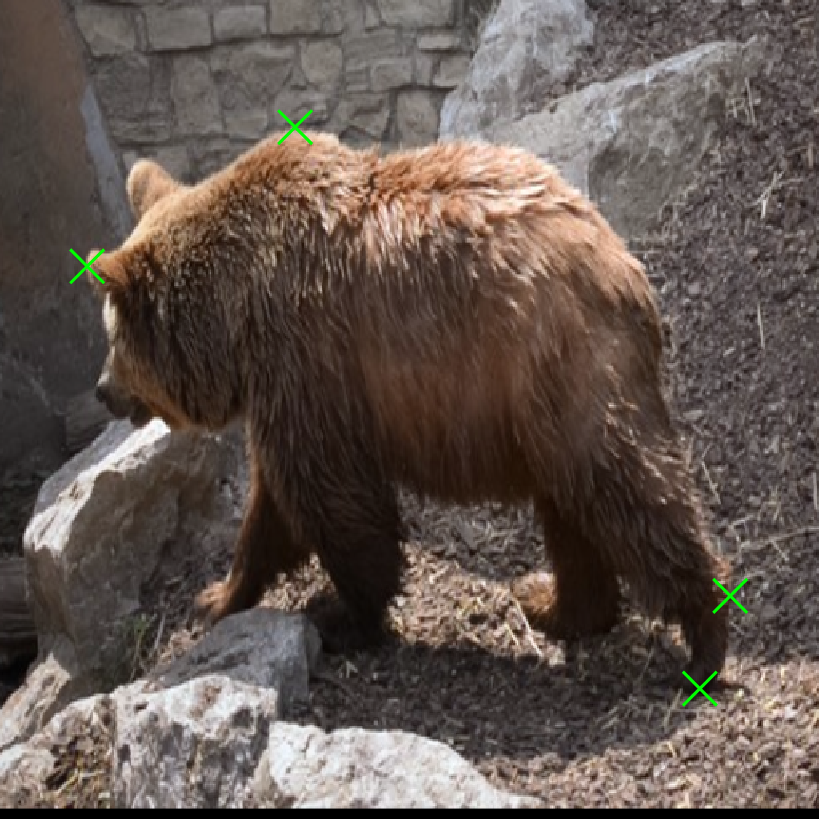
\includegraphics[width=\textwidth]{figures/chap33_channel_rgb.png}
		\caption{RGB image cropped based on the bounding box (three channels).}
		\label{fig:ch3:sec3:rgb_channel}
	\end{subfigure}
	\hfill
	\begin{subfigure}[b]{0.3\textwidth}
		\centering
		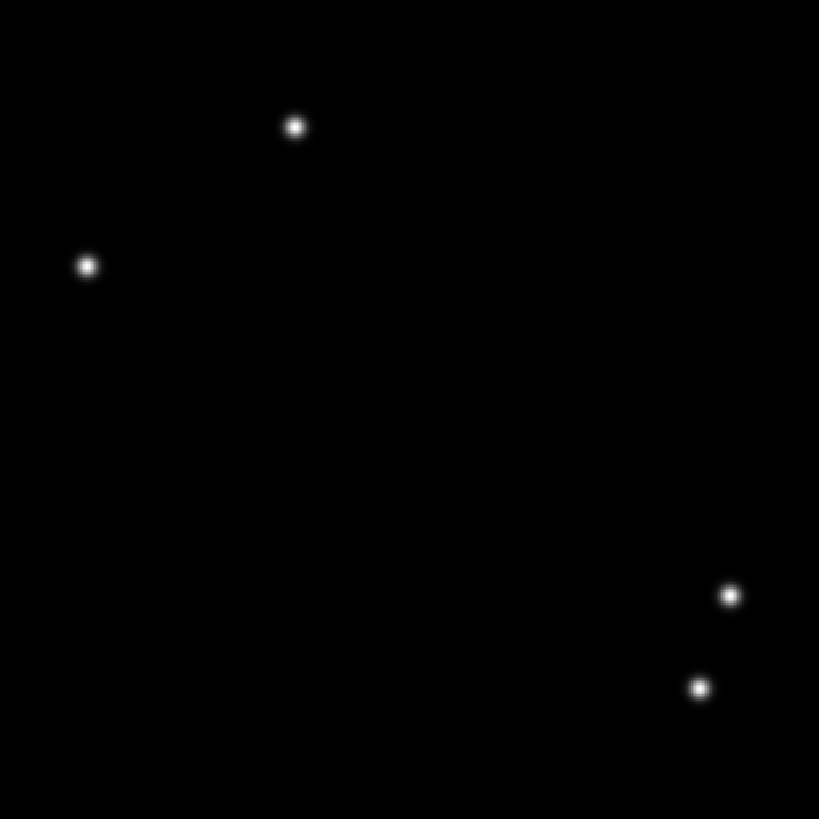
\includegraphics[width=\textwidth]{figures/chap33_channel_fg.png}
		\caption{Foreground heatmap with four extreme points (one channel).}
		\label{fig:ch3:sec3:fg_channel}
	\end{subfigure}
	\hfill
	\begin{subfigure}[b]{0.3\textwidth}
		\centering
		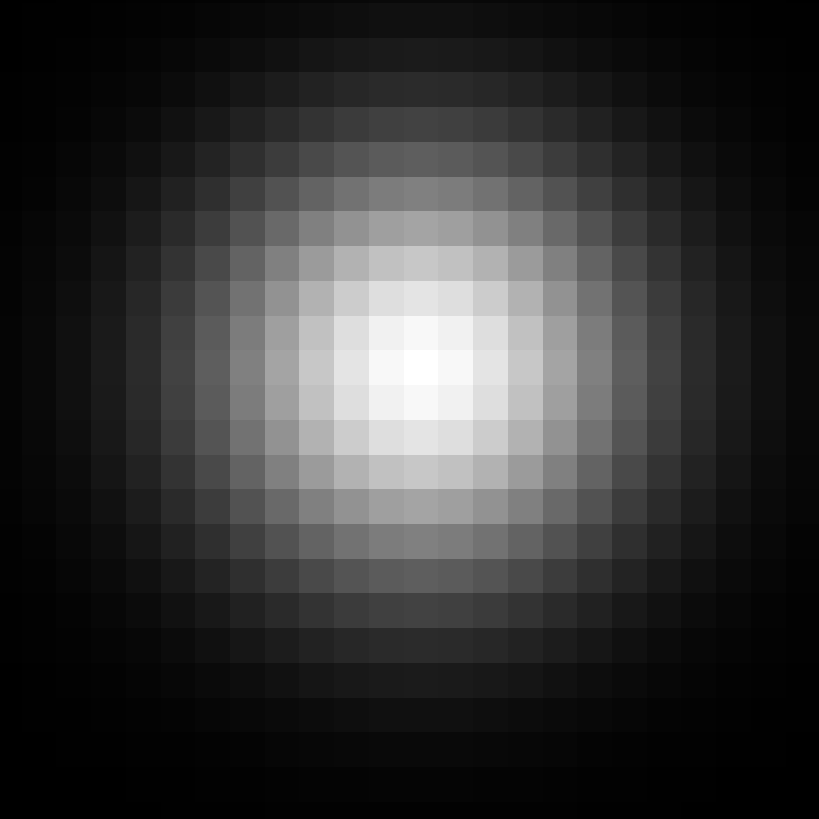
\includegraphics[width=\textwidth]{figures/chap33_gaussian_point.png}
		\caption{Closeup of a point centered with a 2D Gaussian with $\sigma = 10$.}
		\label{fig:ch3:sec3:gauss_centered_point}
	\end{subfigure}
	\caption[Four-channel DEXTR model input]{
		Representation of the separate channels from the four-channel \gls{dextr} model input.
		All channels have the spacial dimension of $512 \times 512$ \Unit{px}.
		The user points on the object's boundary are processed by the 2D Gaussian.
	} \label{fig:ch3:sec3:model_input_channels}
\end{figure}


\subsection{Architecture}\label{ord:ch3:sec3:subsec3}

As encoder for the segmentation network \textit{ResNet-101} \cite{He16-ResNet} is selected, which also referred to as \textit{backbone}.
The ResNet-101 is a deep \gls{cnn} containing 101 layers.
The core components of any ResNets are \textit{residual units}, whose main feature is the use of skip connections \cite{Ger17-HandsOn}.
The ResNet-101 is structured in four blocks, that contain 3, 4, 23 and 3 bottleneck blocks.

The ResNet-101 used for \gls{dextr} is modified by including atrous convolution in the last two blocks and removing the fully connected layers.
After the backbone a four staged \gls{psp} module is applied to preserve global context.
The decoder of this architecture does not consist of several convolution layers, instead bilinear interpolation is used to retrieve original spatial dimension of $512 \times 512$ \Unit{px}.
Finally, a sigmoid function is applied to obtain the final prediction $\textbf{y}$ as a  probability map. \footnote{Wolfram Math world, Sigmoid Function\url{https://mathworld.wolfram.com/SigmoidFunction.html}}

% Training settings.
The model is trained for $ n_{epochs} = 100 $ epochs on the PASCAL \gls{voc} 2012 Segmentation and further $ n_{epochs} = 10 $ epochs on the COCO dataset.
The learning rate is $ \lambda = 10^{-8} $ and the momentum is $ 0.9 $.


\subsection{Refinement}\label{ord:ch3:sec3:subsec4}

As introduced in Subsection \ref{ord:ch2:sec3:subsec2}, some interactive methods provide the possibility to perform refinement, if a segmentation result does not meet the user's expectations.
For the \gls{dextr} method the user may perform refinement by setting an additional click.
The refinement click should be located on the boundary of the region where the segmentation fails.
This new refinement click is added to the foreground heatmap with the extreme points.
In Figure \ref{fig:ch3:sec3:refinement} the effect of an additional refinement click is exemplary presented.
Each refinement click triggers a new model execution.
The refinement process may be applied iteratively.

% TODO plots use an example where the initial prediction actually fails and the refinement succeeds.
\begin{figure} 
	\centering
	\begin{subfigure}[b]{0.45\textwidth}
		\centering
		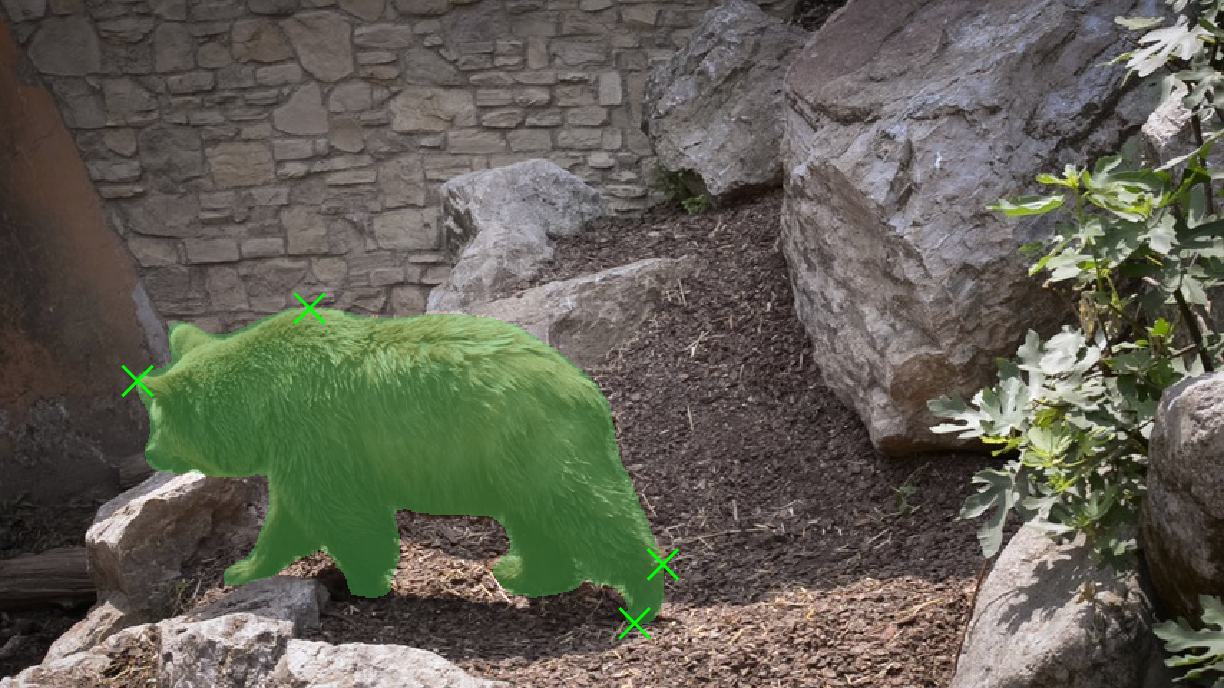
\includegraphics[width=\textwidth]{figures/chap33_bear_initial_result.png}
		\caption{Initial segmentation result.}
		\label{fig:ch3:sec3:refinement_1}
	\end{subfigure}
	\hfill
	\begin{subfigure}[b]{0.45\textwidth}
		\centering
		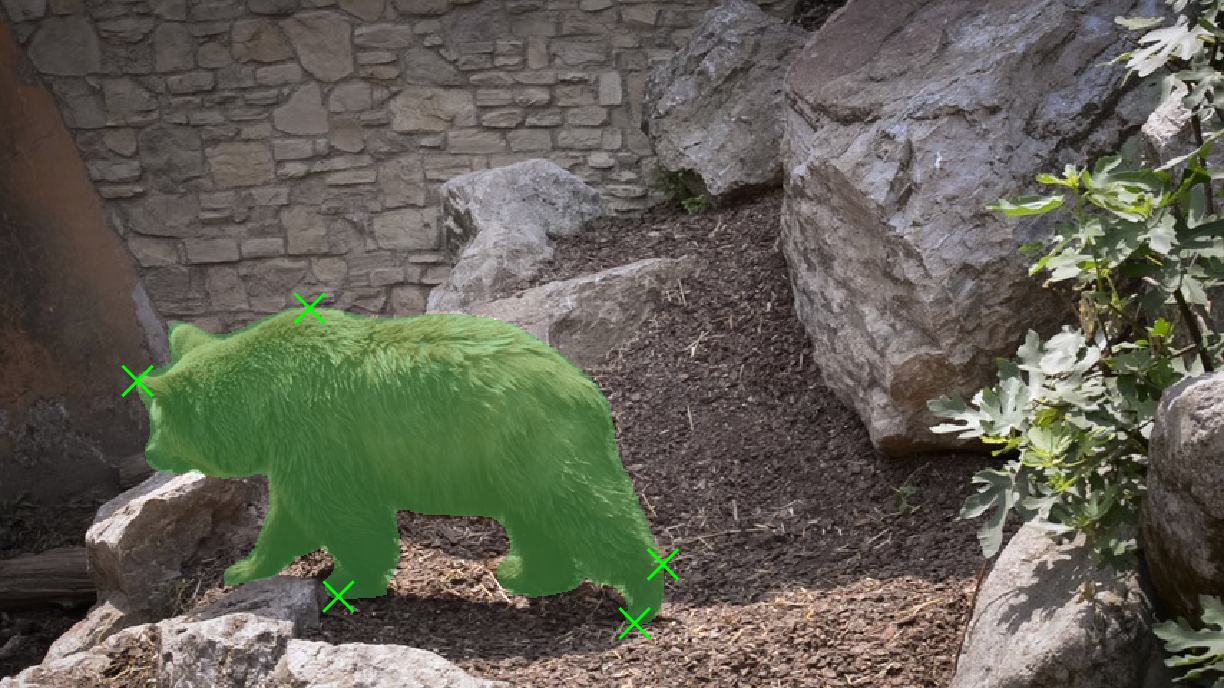
\includegraphics[width=\textwidth]{figures/chap33_bear_refine_result.png}
		\caption{Refinement segmentation result.}
		\label{fig:ch3:sec3:refinement_2}
	\end{subfigure}
	\caption[DEXTR Refinement]{
		On the left is the initial result with the normal extreme points. 
		On the right is the segmentation result with one additional refinement click.
	} \label{fig:ch3:sec3:refinement}
\end{figure}


\subsection{Performance}\label{ord:ch3:sec3:subsec5}

The performance of the \gls{dextr} method in comparison to other interactive segmentation methods in shown in Table \ref{tab:ch2:interactive-stae-of-the-art}.
In this comparison on PASCAL \gls{voc} the \gls{dextr} method performs well and is only outperformed by the \gls{iog} method.

The experiments and evaluations presented in \cite{Man18-DEXTR} contain various datasets and test settings.
Among them is also an examination of the performance on unseen classes and the generalization capability of the method.
Thereby, the model was trained with the PASCAL \gls{voc} or COCO dataset and evaluated on both datasets.
Despite these results seem reliable, it must be taken into account that the PASCAL \gls{voc} and COCO datasets are very similar and cover the same type of \textit{general} objects.
The evaluation of the generalization capabilities of the method continues in detail in Section \ref{ord:ch5:sec2_generalization_image_domains}.

An introduced application for the \gls{dextr} method is to create annotations and use them as new \gls{gt} to train \gls{dl} models.
Manisis \etal claim, that models trained on \gls{dextr} annotations perform equally well as models trained on the original \gls{gt}\cite{Man18-DEXTR}.
This statement is further examined in Section \ref{ord:ch5:sec5_retrain}.
% !TeX root = ../../main.tex
% Add the above to each chapter to make compiling the PDF easier in some editors.

\section{Inside-Outside Guidance}\label{ord:ch3:sec4}

Another approach for interactive segmentation is the \gls{iog} method, introduced in \cite{Zha20-IOG}.
The concept of this state-of-the-art method is strongly based on the previously introduced \gls{dextr} method \cite{Man18-DEXTR}.

\subsection{Basic Concept}\label{ord:ch3:sec4:subsec1}
% User Clicks - Workflow
The user interaction of the \gls{iog} method requires three user clicks executed in two steps.
First, the user has to draw a tight bounding box around the object of interest. 
The drawing of the bounding box may be counted as two user clicks on the background or one stroke.
% TODO refine the stroke possibility
%The creation of the bounding box is implemented using a stroke instead of setting two clicks.
Second, the user has to click once on the center of the object, which is represented as foreground click. 
The described workflow is illustrated in Figure \ref{fig:ch3:sec4:iog_user_clicks}.
Further, the user clicks are processed and an object mask is predicted by a \gls{dl} model.

% Naming of the method
% two-fold
The user provides high level guidance on the foreground and background, representative for the inside and outside region of the object.
On the one hand, this guidance is based on the bounding box that defines the background.
So, everything outside the bounding box does not belong to the object, this is described as \textit{outside} guidance.
On the other hand, the foreground click provides explicit guidance, where the object is located.
This is referred to as \textit{inside} guidance.
These two types of guidance are the namesake of the method \glsentryfull{iog}.
% TODO Auch wenn die Box-Ecken als "background" heatmap verwendet/bezeichnet wird glaube ich, dass das Modell auch lernt, dass sich das Objekt immer innerhalb der Eckpunkte befindet. Die Experimente von Matthias, als er auch mal erlaubt hatte, dass die Box das Objekt nicht ganz überdeckt sind ja glaube ich auch deutlich schlechter ausgefallen. Insofern bieten auch die Box-Eckpunkte eine Art "inside" guidance

% Advantage over DEXTR
Zhang \etal claim, that their way to set user clicks has two advantages compared to the way to set user clicks in other interactive methods as \gls{dextr}.
First, setting of extreme points may be confusing and misleading, as they may be located very close to each other, depending on the orientation of the object.
Second, if the object of interest contains a hole (\eg a donut) or is in the background of another object, \gls{dextr} cannot provide a robust guidance.
In contrast, the variable position of the foreground click in \gls{iog} enables a more robust guidance even for special object scenarios \cite{Zha20-IOG}.

\begin{figure}
	\centering
	\begin{subfigure}[b]{0.3\textwidth}
		\centering
		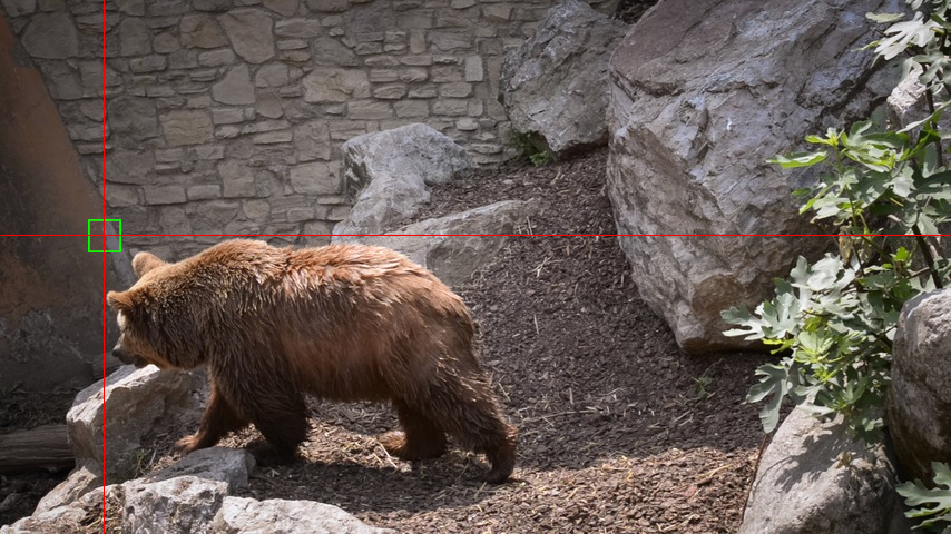
\includegraphics[width=\textwidth]{figures/chap34_bear_2.png}
		\caption{First background click.}
		\label{fig:ch3:sec4:iog_workflow_1}
	\end{subfigure}
	\hfill
	\begin{subfigure}[b]{0.3\textwidth}
		\centering
		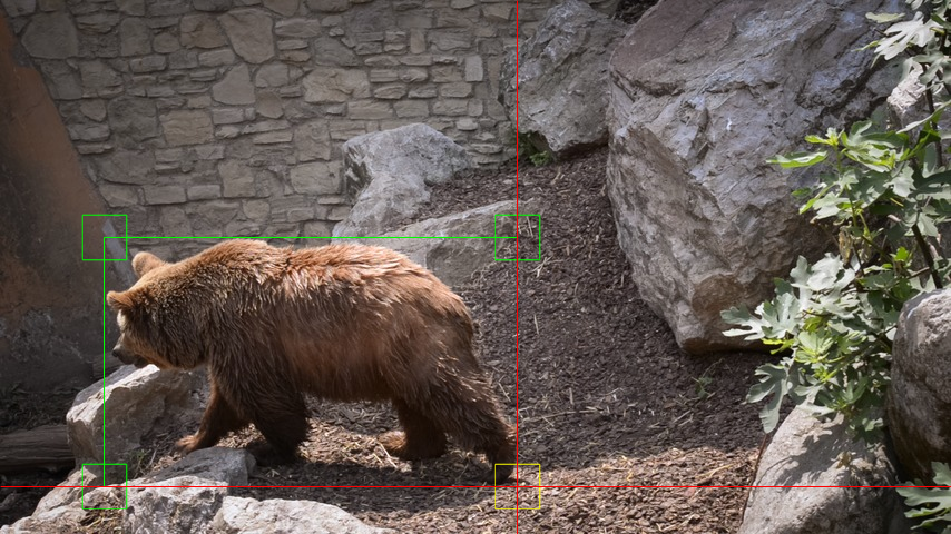
\includegraphics[width=\textwidth]{figures/chap34_bear_3.png}
		\caption{Second background click.}
		\label{fig:ch3:sec4:iog_workflow_2}
	\end{subfigure}
	\hfill
	\begin{subfigure}[b]{0.3\textwidth}
		\centering
		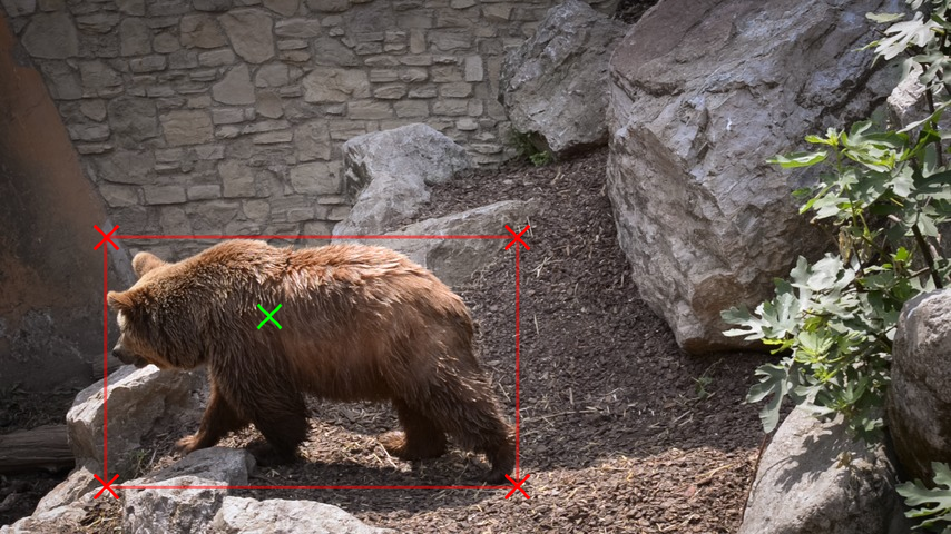
\includegraphics[width=\textwidth]{figures/chap34_bear_5.png}
		\caption{Foreground click.}
		\label{fig:ch3:sec4:iog_workflow_3}
	\end{subfigure}
	\caption[IOG User Interaction]{
		Shown is the workflow to perform the user interaction required for the \gls{iog} method.
		First, a bounding box is spanned by setting two background clicks.
		Last, the foreground click is set.
		All used points are visualized with a cross, background points in red and the foreground point in green, while the contour of the bounding box is drawn in red.
	} 
	\label{fig:ch3:sec4:iog_user_clicks}
\end{figure}

\subsection{Model Input and Representation of User Clicks}\label{ord:ch3:sec4:subsec2}

Identical to the \gls{dextr} method, the background clicks form a bounding box, which is enlarged by  $p_{{box}}$ \Unit{px}.
This processing is identical to the \gls{dextr} method.
% TODO ??mention that the background points are move by ~10 pixel in order to avoid the enforced background points being on the foreground
The image is cropped based on the enlarged bounding box and resized to the size of $512 \times 512$ \Unit{px}, if necessary zero padding is applied.

The bounding box is formed by the two background points, that are diagonal corners points (top-left and bottom-right or bottom-left and top-right).
Based on these two points, the other two corner points are derived, which provides four background points for the price of two.
As in the \gls{dextr} processing, the fore- and background clicks are converted into points on two separate heatmaps.
To highlight the user points a 2D Gaussian is centered around each click (see Equation \ref{equ:gauss}).

The two heatmaps have the size of $512 \times 512$ \Unit{px} and are concatenated with the \Gls{rgb} image.
This results in the five-channel \gls{iog} model input, which is explanatory illustrated in Figure \ref{fig:ch3:sec4:model_input_channels}.

%TODO add crosses to cropped RGB image
\begin{figure}
	\centering
	\begin{subfigure}[b]{0.3\textwidth}
		\centering
		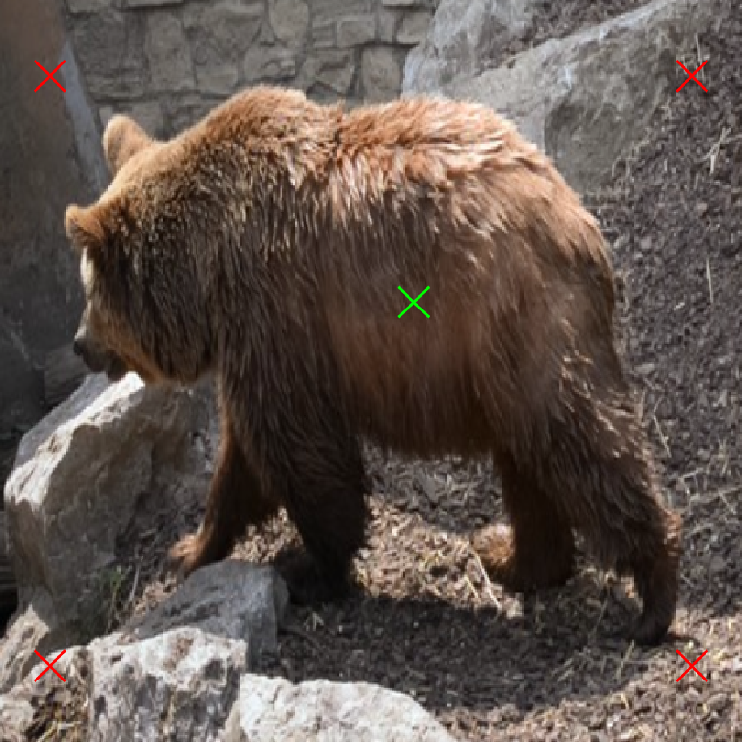
\includegraphics[width=\textwidth]{figures/chap34_channel_rgb.png}
		\caption{RGB image cropped based on the bounding box (three channels).}
		\label{fig:ch3:sec4:rgb_channel}
	\end{subfigure}
	\hfill
	\begin{subfigure}[b]{0.3\textwidth}
		\centering
		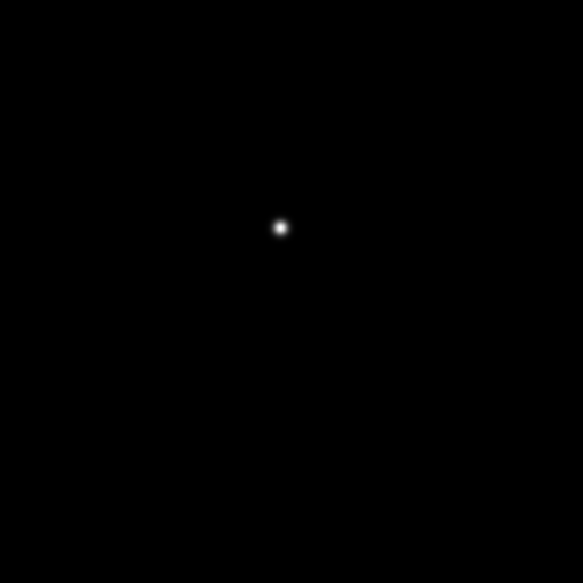
\includegraphics[width=\textwidth]{figures/chap34_channel_fg.png}
		\caption{Foreground heatmap with one foreground point (one channel).}
		\label{fig:ch3:sec4:fg_channel}
	\end{subfigure}
	\hfill
	\begin{subfigure}[b]{0.3\textwidth}
		\centering
		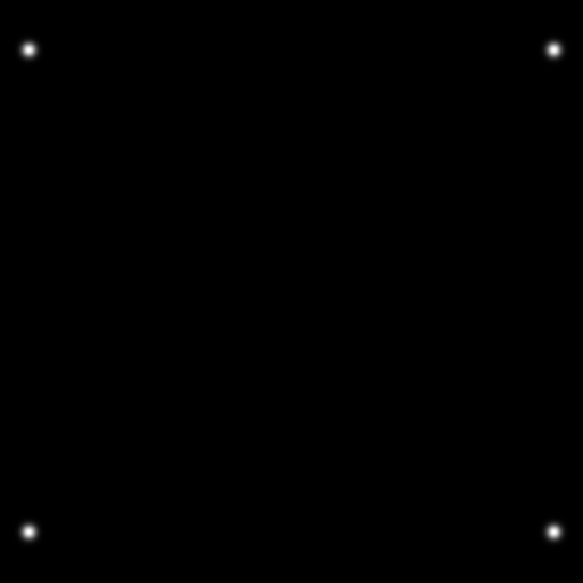
\includegraphics[width=\textwidth]{figures/chap34_channel_bg.png}
		\caption{Background heatmap with four background points (one channel).}
		\label{fig:ch3:sec4:bg_channel}
	\end{subfigure}
	\caption[Five-channel IOG model input]{
		Representation of the separate channels from the five-channel \gls{iog} model input.
		All channels have the spatial dimension of $512 \times 512$ \Unit{px}.
		The user points in the foreground and background heatmaps are enforced with a 2D Gaussian.
	} \label{fig:ch3:sec4:model_input_channels}
\end{figure}

\subsection{Architecture}\label{ord:ch3:sec4:subsec3}

The model architecture used for the \gls{iog} method is based on the encoder-decoder architecture and special structure for layer fusion.
The encoder-decoder network is titled as \textit{CoraseNet}, while the structure for layer fusion is referred to as \textit{FineNet}.
An illustration of the complete architecture is given in Figure \ref{fig:ch3:sec4:arch}.


\subsubsection{CoarseNet}
The CoarseNet consists out of multiple components: encoder network, decoder network, \gls{psp}-module and skip connections. The CoarseNet is built upon the \gls{dextr} method, therefore they partially share the same architectural components.

As in the \gls{dextr} architecture, the encoder network is represented by ResNet-101 \cite{He16-ResNet}, followed by a \gls{psp} module.
%The ResNet is implemented without the head of fully connected layers. It contains four ResNet blocks and the fourth block outputs 2048 feature maps of the size $32 \times 32$ \Unit{px}.
% As in \gls{dextr} a \gls{psp}-module is applied after the backbone to gain more contextual information.
The output of the \gls{psp}-module is a coarse prediction with the spatial dimension of  $32 \times 32$ \Unit{px} containing 512 feature maps. 

From this onward the decoder network starts the upsampling process.
% TODO declare what kind of operations are used for the upsampling.
The decoder network is built upon a reversed, simplified version of the encoder architecture. % , that consists out of four residual blocks.
Therefore, the decoder network is based on four blocks, in order to regain the original input size of  $512 \times 512$ \Unit{px}.
Further, three skip connection are applied and establish a connection in between the four resiudual blocks of the encoder and decoder network, as visualized in Figure \ref{fig:ch3:sec4:arch}.
% TODO this skip connection also does some processing
% During the upsampling process activations from the residual blocks of the ResNet are transferred from the ResNet using so lateral connections and concatenated with the upsampled feature maps.
% A benefit of this architecture is the fusion of information from different network stages.
\begin{figure}
	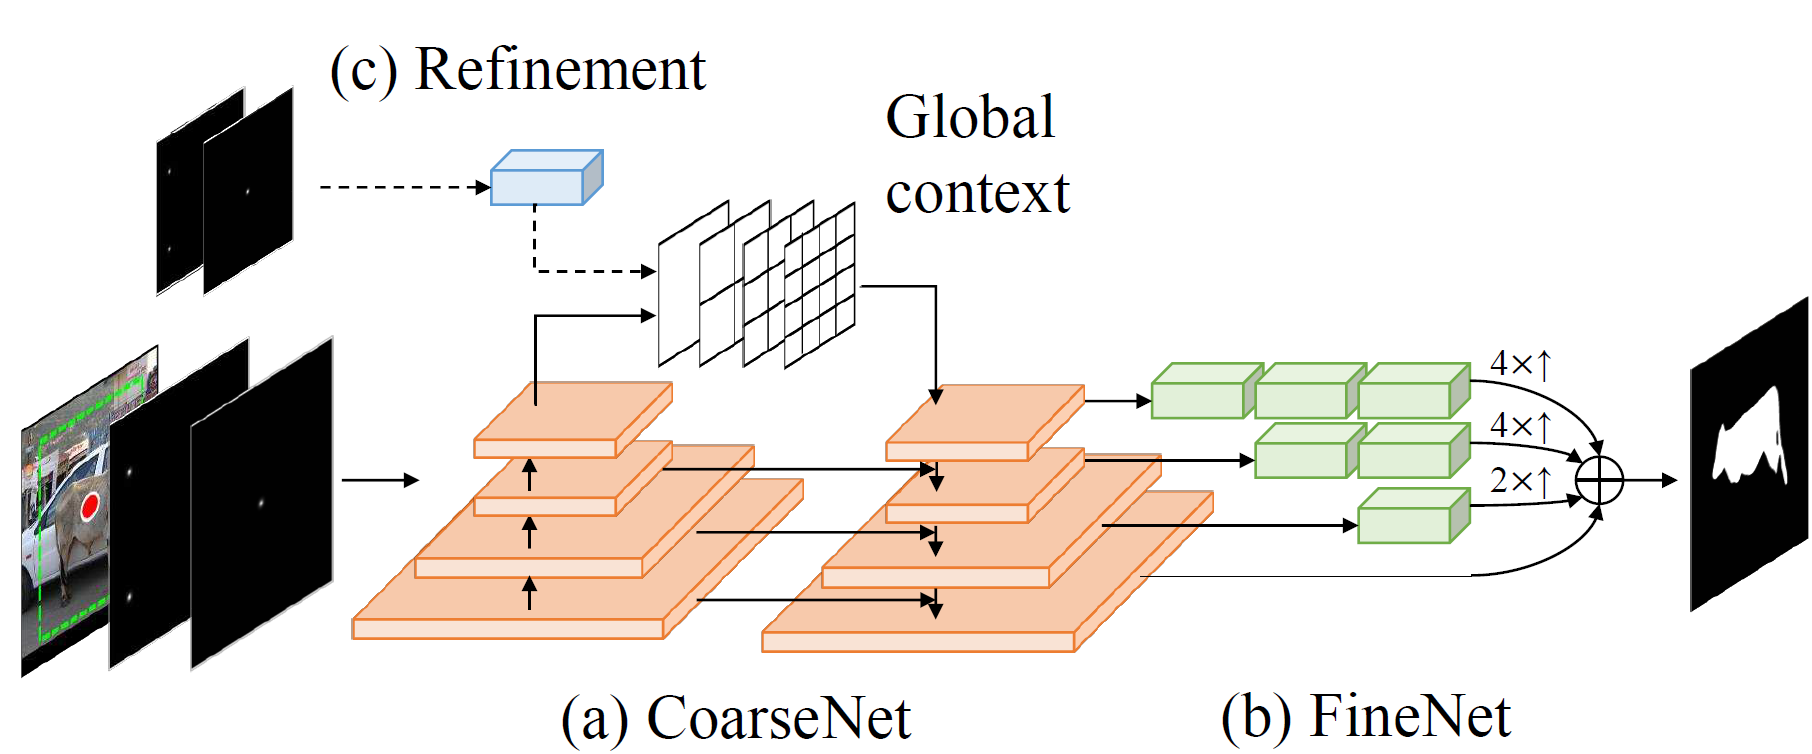
\includegraphics[width=\linewidth]{figures/chap34_iog_arch.png}
	\caption[IOG Architecture]{		
		Architecture of the \gls{iog} model.
		On the left the model input is visualized as in Figure \ref{fig:ch3:sec4:model_input_channels}.
		The CoarseNet is marked by (a) and shows the encoder and decoder network with the skip connections and the \gls{psp} module.
		The FineNet is marked by (b) and represents the four stream fusion structure.
		It can be seen, that the single streams origin from different levels of the decoder network.
		In order to obtain a common spatial dimension for concatenation $ \oplus $, the streams differ in their processing.
		As final prediction a binary object mask is shown.
		The lightweight-branch for refinement is marked with (c).
		Copyright \copyright 2020 IEEE. Reprinted by permission from \cite{Zha20-IOG}.
	}
	\label{fig:ch3:sec4:arch}
\end{figure}

\subsubsection{FineNet}
The FineNet consists of a four-stream fusion structure.
The four streams originate from the four levels of the decoder network and, therefore, process feature maps of various sizes (see Figure \ref{fig:ch3:sec4:arch}).
Each stream processes and upsamples the feature maps by a descending number of bottleneck processing blocks.
The streams reconstruct the feature maps to the final spatial dimension of $512 \times 512$ \Unit{px}.
%applied in order to use \emph{"features at deeper layers for better trade-off between accuracy and efficiency"} \cite[p. 12237]{Zha20-IOG}.
In the end the four streams are concatenated and pass through a final bottleneck processing block.
To the final output a sigmoid is applied, which results in a probability map as final prediction of the \gls{iog} network.

The author justifies the application of these different components by showing their effect in an ablation study \cite{Zha20-IOG}.
% The author shows in an ablation study, that the FineNet enhances the networks IoU by $0.8\%$. 
% The ablation study is performed with a ResNet-50 as backbone and PASCAL-1k \cite{Eve20-PascalVOC} as dataset. 


\subsection{Refinement}\label{ord:ch3:sec4:subsec4}

To perform refinement in the \gls{iog} method, the user sets an additional click on the largest fore- or background region that was predicted wrongly.
Identically to the \gls{dextr} method, refinement may be performed iteratively and each refinement click triggers a model execution.
However, in contrast to \gls{dextr} the refinement of the \gls{iog} method does not require the execution of the complete model, but just the refinement part the FineNet.

The integration in the existing architecture is realized as follows.
New heatmaps for fore- and background are created with the original clicks and the refinement clicks.
These two heatmaps are combined into a two-channel input, which is processed in a so called lightweight-branch.
This lightweight-branch consists out of five convolutional layers, that perform the downsampling.
The output of this branch is combined with the output of the initial iteration from the encoder network and forwarded to the \gls{psp} module as shown in Figure \ref{fig:ch3:sec4:arch}.
This means that the computationally expensive encoder must only be executed for the initial prediction.
From the \gls{psp} module onwards the model is executed normally.

Hence, the encoder network does not require a new execution and the execution of the model time is decreased.
Zhang \etal state, that the usage of the lightweight-branch performs better than directly adding the refinement click into the normal five-channel input.

% TODO use an example where the initial prediction actually fails and the refinement succeeds.
\begin{figure} 
	\centering
	\begin{subfigure}[b]{0.45\textwidth}
		\centering
		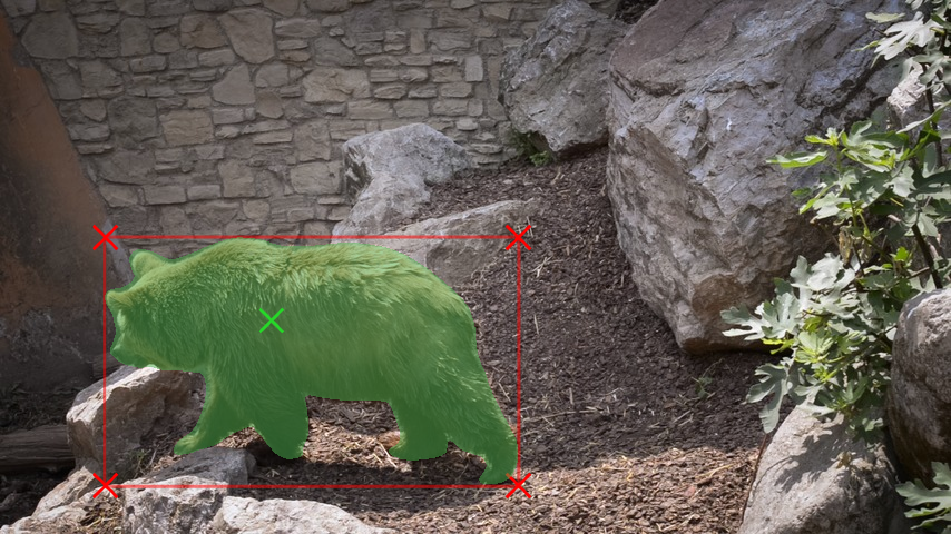
\includegraphics[width=\textwidth]{figures/chap34_bear_6.png}
		\caption{Initial segmentation result.}
		\label{fig:ch3:sec4:refinement_1}
	\end{subfigure}
	\hfill
	\begin{subfigure}[b]{0.45\textwidth}
		\centering
		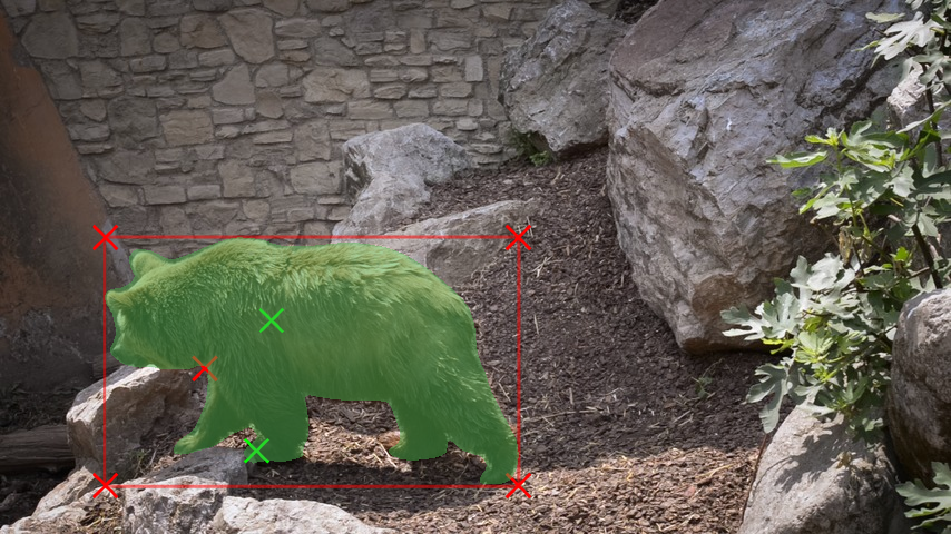
\includegraphics[width=\textwidth]{figures/chap34_bear_8.png}
		\caption{Refinement segmentation result.}
		\label{fig:ch3:sec4:refinement_2}
	\end{subfigure}
	\caption[IOG Refinement]{
		On the left is the initial result with the normal amount of clicks. 
		On the right is the results of two refinement iterations with one additional refinement click on the foreground and one on the background.
	} \label{fig:ch3:sec4:refinement}
\end{figure}


\subsection{Performance}\label{ord:ch3:sec4:subsec5}

An overview of interactive segmentation methods is presented in Table \ref{tab:ch2:interactive-stae-of-the-art}.
It can be seen that the \gls{iog} outperforms other state-of-the-art methods with respect to the number of set points to reach a certain IoU-level and the achieved \gls{iou} at exactly four clicks.

% TODO Comment von Paddo - Ist das etwas was du rausgefunden hast oder steht das so im Paper oder ist das deine Intuition? 
This method especially performs well due the highly connected architecture.
The application of skip connections and the FineNet enable the model to recover local details and prevent the information loss during down- and upsampling process.

Similar to the experiments performed in \cite{Man18-DEXTR}, Zhang \etal also investigate the performance on unseen classes and the generalization capability of the method \Cite{Zha20-IOG}. 
This topic will be continued by the evaluation of other unseen domains in Section \ref{ord:ch5:sec2_generalization_domains}.

Zhang \etal also evaluate the performance on dataset with other domains than PASCAL \gls{voc} (\eg Rooftops, CityScapes, or Agricultural-Vision).
Further, it is demonstated in various setups, that the \gls{iog} method trained on PASCAL \gls{voc} outperformed the \gls{dextr} method or the \textit{Curve-\gls{gcn}}, both trained on the CityScapes dataset.

% TODO appendix with various examples of IOG segmentation results?

% TODO: add more chapters here
\appendix{}

\microtypesetup{protrusion=false}
\listoffigures{}
\listoftables{}
\microtypesetup{protrusion=true}
%\printglossary[type=acronymtype, nonumberlist] % type=main,style=long
\printglossaries{}
%\printacronyms{}
\printbibliography{}

\end{document}
